\documentclass[1p]{elsarticle_modified}
%\bibliographystyle{elsarticle-num}

%\usepackage[colorlinks]{hyperref}
%\usepackage{abbrmath_seonhwa} %\Abb, \Ascr, \Acal ,\Abf, \Afrak
\usepackage{amsfonts}
\usepackage{amssymb}
\usepackage{amsmath}
\usepackage{amsthm}
\usepackage{scalefnt}
\usepackage{amsbsy}
\usepackage{kotex}
\usepackage{caption}
\usepackage{subfig}
\usepackage{color}
\usepackage{graphicx}
\usepackage{xcolor} %% white, black, red, green, blue, cyan, magenta, yellow
\usepackage{float}
\usepackage{setspace}
\usepackage{hyperref}

\usepackage{tikz}
\usetikzlibrary{arrows}

\usepackage{multirow}
\usepackage{array} % fixed length table
\usepackage{hhline}

%%%%%%%%%%%%%%%%%%%%%
\makeatletter
\renewcommand*\env@matrix[1][\arraystretch]{%
	\edef\arraystretch{#1}%
	\hskip -\arraycolsep
	\let\@ifnextchar\new@ifnextchar
	\array{*\c@MaxMatrixCols c}}
\makeatother %https://tex.stackexchange.com/questions/14071/how-can-i-increase-the-line-spacing-in-a-matrix
%%%%%%%%%%%%%%%

\usepackage[normalem]{ulem}

\newcommand{\msout}[1]{\ifmmode\text{\sout{\ensuremath{#1}}}\else\sout{#1}\fi}
%SOURCE: \msout is \stkout macro in https://tex.stackexchange.com/questions/20609/strikeout-in-math-mode

\newcommand{\cancel}[1]{
	\ifmmode
	{\color{red}\msout{#1}}
	\else
	{\color{red}\sout{#1}}
	\fi
}

\newcommand{\add}[1]{
	{\color{blue}\uwave{#1}}
}

\newcommand{\replace}[2]{
	\ifmmode
	{\color{red}\msout{#1}}{\color{blue}\uwave{#2}}
	\else
	{\color{red}\sout{#1}}{\color{blue}\uwave{#2}}
	\fi
}

\newcommand{\Sol}{\mathcal{S}} %segment
\newcommand{\D}{D} %diagram
\newcommand{\A}{\mathcal{A}} %arc


%%%%%%%%%%%%%%%%%%%%%%%%%%%%%5 test

\def\sl{\operatorname{\textup{SL}}(2,\Cbb)}
\def\psl{\operatorname{\textup{PSL}}(2,\Cbb)}
\def\quan{\mkern 1mu \triangleright \mkern 1mu}

\theoremstyle{definition}
\newtheorem{thm}{Theorem}[section]
\newtheorem{prop}[thm]{Proposition}
\newtheorem{lem}[thm]{Lemma}
\newtheorem{ques}[thm]{Question}
\newtheorem{cor}[thm]{Corollary}
\newtheorem{defn}[thm]{Definition}
\newtheorem{exam}[thm]{Example}
\newtheorem{rmk}[thm]{Remark}
\newtheorem{alg}[thm]{Algorithm}

\newcommand{\I}{\sqrt{-1}}
\begin{document}

%\begin{frontmatter}
%
%\title{Boundary parabolic representations of knots up to 8 crossings}
%
%%% Group authors per affiliation:
%\author{Yunhi Cho} 
%\address{Department of Mathematics, University of Seoul, Seoul, Korea}
%\ead{yhcho@uos.ac.kr}
%
%
%\author{Seonhwa Kim} %\fnref{s_kim}}
%\address{Center for Geometry and Physics, Institute for Basic Science, Pohang, 37673, Korea}
%\ead{ryeona17@ibs.re.kr}
%
%\author{Hyuk Kim}
%\address{Department of Mathematical Sciences, Seoul National University, Seoul 08826, Korea}
%\ead{hyukkim@snu.ac.kr}
%
%\author{Seokbeom Yoon}
%\address{Department of Mathematical Sciences, Seoul National University, Seoul, 08826,  Korea}
%\ead{sbyoon15@snu.ac.kr}
%
%\begin{abstract}
%We find all boundary parabolic representation of knots up to 8 crossings.
%
%\end{abstract}
%\begin{keyword}
%    \MSC[2010] 57M25 
%\end{keyword}
%
%\end{frontmatter}

%\linenumbers
%\tableofcontents
%
\newcommand\colored[1]{\textcolor{white}{\rule[-0.35ex]{0.8em}{1.4ex}}\kern-0.8em\color{red} #1}%
%\newcommand\colored[1]{\textcolor{white}{ #1}\kern-2.17ex	\textcolor{white}{ #1}\kern-1.81ex	\textcolor{white}{ #1}\kern-2.15ex\color{red}#1	}

{\Large $\underline{12a_{0088}~(K12a_{0088})}$}

\setlength{\tabcolsep}{10pt}
\renewcommand{\arraystretch}{1.6}
\vspace{1cm}\begin{tabular}{m{100pt}>{\centering\arraybackslash}m{274pt}}
\multirow{5}{120pt}{
	\centering
	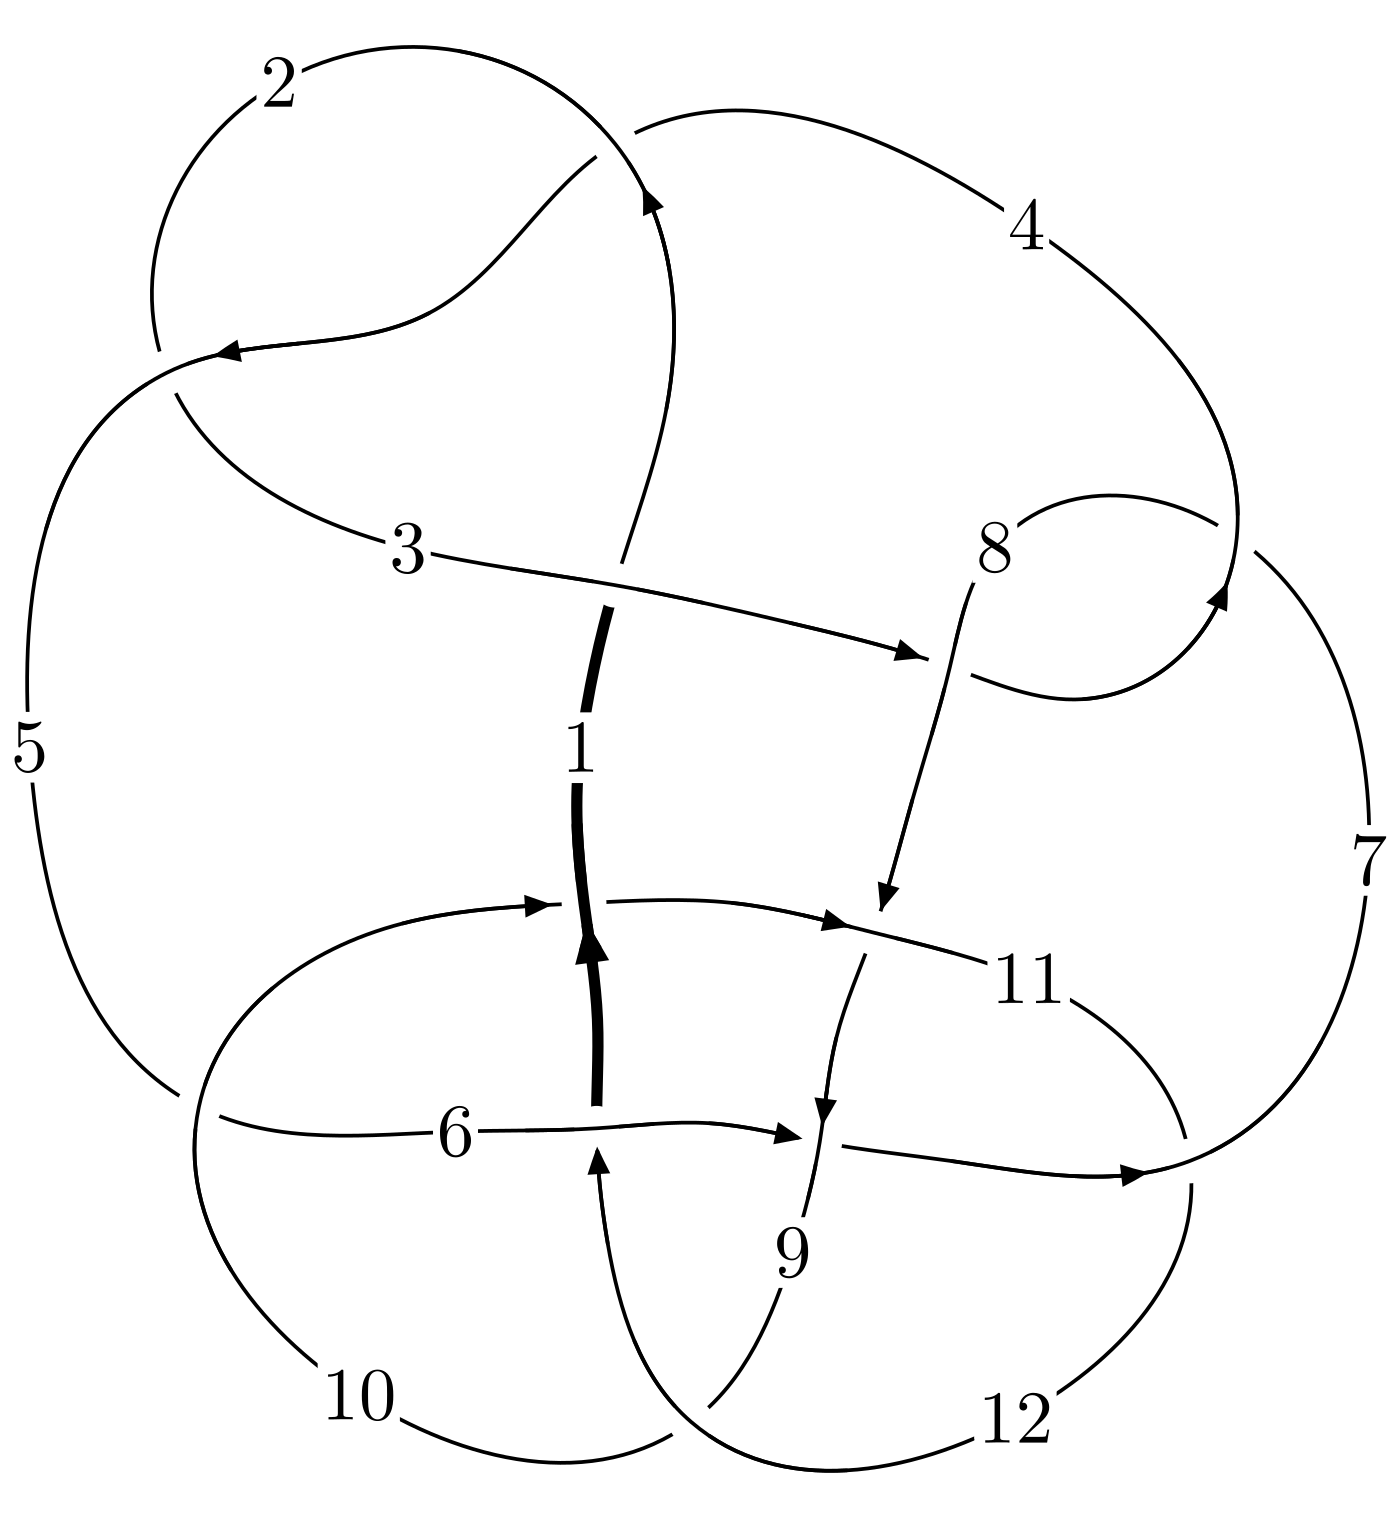
\includegraphics[width=112pt]{../../../GIT/diagram.site/Diagrams/png/889_12a_0088.png}\\
\ \ \ A knot diagram\footnotemark}&
\allowdisplaybreaks
\textbf{Linearized knot diagam} \\
\cline{2-2}
 &
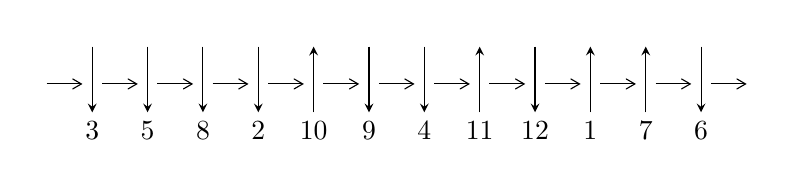
\begin{tikzpicture}[x=20pt, y=17pt]
	% nodes
	\node (C0) at (0, 0) {};
	\node (C1) at (1, 0) {};
	\node (C1U) at (1, +1) {};
	\node (C1D) at (1, -1) {3};

	\node (C2) at (2, 0) {};
	\node (C2U) at (2, +1) {};
	\node (C2D) at (2, -1) {5};

	\node (C3) at (3, 0) {};
	\node (C3U) at (3, +1) {};
	\node (C3D) at (3, -1) {8};

	\node (C4) at (4, 0) {};
	\node (C4U) at (4, +1) {};
	\node (C4D) at (4, -1) {2};

	\node (C5) at (5, 0) {};
	\node (C5U) at (5, +1) {};
	\node (C5D) at (5, -1) {10};

	\node (C6) at (6, 0) {};
	\node (C6U) at (6, +1) {};
	\node (C6D) at (6, -1) {9};

	\node (C7) at (7, 0) {};
	\node (C7U) at (7, +1) {};
	\node (C7D) at (7, -1) {4};

	\node (C8) at (8, 0) {};
	\node (C8U) at (8, +1) {};
	\node (C8D) at (8, -1) {11};

	\node (C9) at (9, 0) {};
	\node (C9U) at (9, +1) {};
	\node (C9D) at (9, -1) {12};

	\node (C10) at (10, 0) {};
	\node (C10U) at (10, +1) {};
	\node (C10D) at (10, -1) {1};

	\node (C11) at (11, 0) {};
	\node (C11U) at (11, +1) {};
	\node (C11D) at (11, -1) {7};

	\node (C12) at (12, 0) {};
	\node (C12U) at (12, +1) {};
	\node (C12D) at (12, -1) {6};
	\node (C13) at (13, 0) {};

	% arrows
	\draw[->,>={angle 60}]
	(C0) edge (C1) (C1) edge (C2) (C2) edge (C3) (C3) edge (C4) (C4) edge (C5) (C5) edge (C6) (C6) edge (C7) (C7) edge (C8) (C8) edge (C9) (C9) edge (C10) (C10) edge (C11) (C11) edge (C12) (C12) edge (C13) ;	\draw[->,>=stealth]
	(C1U) edge (C1D) (C2U) edge (C2D) (C3U) edge (C3D) (C4U) edge (C4D) (C5D) edge (C5U) (C6U) edge (C6D) (C7U) edge (C7D) (C8D) edge (C8U) (C9U) edge (C9D) (C10D) edge (C10U) (C11D) edge (C11U) (C12U) edge (C12D) ;
	\end{tikzpicture} \\
\hhline{~~} \\& 
\textbf{Solving Sequence} \\ \cline{2-2} 
 &
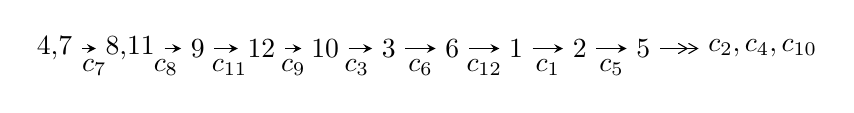
\begin{tikzpicture}[x=23pt, y=7pt]
	% node
	\node (A0) at (-1/8, 0) {4,7};
	\node (A1) at (17/16, 0) {8,11};
	\node (A2) at (17/8, 0) {9};
	\node (A3) at (25/8, 0) {12};
	\node (A4) at (33/8, 0) {10};
	\node (A5) at (41/8, 0) {3};
	\node (A6) at (49/8, 0) {6};
	\node (A7) at (57/8, 0) {1};
	\node (A8) at (65/8, 0) {2};
	\node (A9) at (73/8, 0) {5};
	\node (C1) at (1/2, -1) {$c_{7}$};
	\node (C2) at (13/8, -1) {$c_{8}$};
	\node (C3) at (21/8, -1) {$c_{11}$};
	\node (C4) at (29/8, -1) {$c_{9}$};
	\node (C5) at (37/8, -1) {$c_{3}$};
	\node (C6) at (45/8, -1) {$c_{6}$};
	\node (C7) at (53/8, -1) {$c_{12}$};
	\node (C8) at (61/8, -1) {$c_{1}$};
	\node (C9) at (69/8, -1) {$c_{5}$};
	\node (A10) at (11, 0) {$c_{2},c_{4},c_{10}$};

	% edge
	\draw[->,>=stealth]	
	(A0) edge (A1) (A1) edge (A2) (A2) edge (A3) (A3) edge (A4) (A4) edge (A5) (A5) edge (A6) (A6) edge (A7) (A7) edge (A8) (A8) edge (A9) ;
	\draw[->>,>={angle 60}]	
	(A9) edge (A10);
\end{tikzpicture} \\ 

\end{tabular} \\

\footnotetext{
The image of knot diagram is generated by the software ``\textbf{Draw programme}" developed by Andrew Bartholomew(\url{http://www.layer8.co.uk/maths/draw/index.htm\#Running-draw}), where we modified some parts for our purpose(\url{https://github.com/CATsTAILs/LinksPainter}).
}\phantom \\ \newline 
\centering \textbf{Ideals for irreducible components\footnotemark of $X_{\text{par}}$} 
 
\begin{align*}
I^u_{1}&=\langle 
3.50265\times10^{167} u^{75}+1.62291\times10^{168} u^{74}+\cdots+2.17923\times10^{168} b-2.92816\times10^{168},\\
\phantom{I^u_{1}}&\phantom{= \langle  }1.34711\times10^{170} u^{75}+3.31466\times10^{170} u^{74}+\cdots+5.57883\times10^{170} a+2.14734\times10^{172},\\
\phantom{I^u_{1}}&\phantom{= \langle  }u^{76}+5 u^{75}+\cdots-1504 u-256\rangle \\
I^u_{2}&=\langle 
5.40539\times10^{57} a u^{53}+5.21405\times10^{57} u^{53}+\cdots+2.28078\times10^{59} a+9.87330\times10^{58},\\
\phantom{I^u_{2}}&\phantom{= \langle  }2.49928\times10^{59} a u^{53}+5.44370\times10^{58} u^{53}+\cdots-9.46034\times10^{59} a+3.73776\times10^{60},\;u^{54}-2 u^{53}+\cdots-36 u+8\rangle \\
I^u_{3}&=\langle 
768246826 u^{22}-1643416610 u^{21}+\cdots+219374557 b+473494586,\\
\phantom{I^u_{3}}&\phantom{= \langle  }99816722 u^{22}+500697163 u^{21}+\cdots+219374557 a+85184191,\;u^{23}-2 u^{22}+\cdots+u-1\rangle \\
I^u_{4}&=\langle 
- u^2 a+b+1,\;-4 u^2 a+a^2-2 a u+8 u^2-5 a+3 u+15,\;u^3+u^2+2 u+1\rangle \\
\\
I^v_{1}&=\langle 
a,\;16 v^3-48 v^2+b+51 v-13,\;4 v^4-13 v^3+16 v^2-7 v+1\rangle \\
I^v_{2}&=\langle 
a,\;b^2- b v+v^2- b+2 v+2,\;v^3+2 v^2+3 v+1\rangle \\
\end{align*}
\raggedright * 6 irreducible components of $\dim_{\mathbb{C}}=0$, with total 223 representations.\\
\footnotetext{All coefficients of polynomials are rational numbers. But the coefficients are sometimes approximated in decimal forms when there is not enough margin.}
\newpage
\renewcommand{\arraystretch}{1}
\centering \section*{I. $I^u_{1}= \langle 3.50\times10^{167} u^{75}+1.62\times10^{168} u^{74}+\cdots+2.18\times10^{168} b-2.93\times10^{168},\;1.35\times10^{170} u^{75}+3.31\times10^{170} u^{74}+\cdots+5.58\times10^{170} a+2.15\times10^{172},\;u^{76}+5 u^{75}+\cdots-1504 u-256 \rangle$}
\flushleft \textbf{(i) Arc colorings}\\
\begin{tabular}{m{7pt} m{180pt} m{7pt} m{180pt} }
\flushright $a_{4}=$&$\begin{pmatrix}0\\u\end{pmatrix}$ \\
\flushright $a_{7}=$&$\begin{pmatrix}1\\0\end{pmatrix}$ \\
\flushright $a_{8}=$&$\begin{pmatrix}1\\u^2\end{pmatrix}$ \\
\flushright $a_{11}=$&$\begin{pmatrix}-0.241468 u^{75}-0.594150 u^{74}+\cdots-211.857 u-38.4908\\-0.160728 u^{75}-0.744715 u^{74}+\cdots+69.1978 u+1.34366\end{pmatrix}$ \\
\flushright $a_{9}=$&$\begin{pmatrix}0.429938 u^{75}+2.37634 u^{74}+\cdots-882.782 u-147.812\\-0.499536 u^{75}-2.13504 u^{74}+\cdots+443.772 u+61.6431\end{pmatrix}$ \\
\flushright $a_{12}=$&$\begin{pmatrix}-0.402196 u^{75}-1.33887 u^{74}+\cdots-142.659 u-37.1472\\-0.160728 u^{75}-0.744715 u^{74}+\cdots+69.1978 u+1.34366\end{pmatrix}$ \\
\flushright $a_{10}=$&$\begin{pmatrix}-0.249605 u^{75}-1.21879 u^{74}+\cdots+592.443 u+125.818\\-0.221325 u^{75}-1.11335 u^{74}+\cdots+502.440 u+98.4113\end{pmatrix}$ \\
\flushright $a_{3}=$&$\begin{pmatrix}u\\u^3+u\end{pmatrix}$ \\
\flushright $a_{6}=$&$\begin{pmatrix}-0.0578480 u^{75}-0.146509 u^{74}+\cdots-107.825 u-25.7212\\0.212028 u^{75}+0.991418 u^{74}+\cdots-455.593 u-89.2052\end{pmatrix}$ \\
\flushright $a_{1}=$&$\begin{pmatrix}-0.449045 u^{75}-1.77037 u^{74}+\cdots+239.294 u+44.5157\\0.126005 u^{75}+0.424987 u^{74}+\cdots-38.9179 u+13.2441\end{pmatrix}$ \\
\flushright $a_{2}=$&$\begin{pmatrix}-0.0856491 u^{75}-0.525662 u^{74}+\cdots+361.435 u+92.6534\\0.762094 u^{75}+3.29215 u^{74}+\cdots-684.443 u-85.1196\end{pmatrix}$ \\
\flushright $a_{5}=$&$\begin{pmatrix}-0.627609 u^{75}-2.95001 u^{74}+\cdots+877.437 u+152.834\\-0.178564 u^{75}-1.17964 u^{74}+\cdots+638.143 u+108.319\end{pmatrix}$\\&\end{tabular}
\flushleft \textbf{(ii) Obstruction class $= -1$}\\~\\
\flushleft \textbf{(iii) Cusp Shapes $= 0.630979 u^{75}+1.28928 u^{74}+\cdots+1959.31 u+521.805$}\\~\\
\newpage\renewcommand{\arraystretch}{1}
\flushleft \textbf{(iv) u-Polynomials at the component}\newline \\
\begin{tabular}{m{50pt}|m{274pt}}
Crossings & \hspace{64pt}u-Polynomials at each crossing \\
\hline $$\begin{aligned}c_{1}\end{aligned}$$&$\begin{aligned}
&u^{76}+41 u^{75}+\cdots+2881 u+256
\end{aligned}$\\
\hline $$\begin{aligned}c_{2},c_{4}\end{aligned}$$&$\begin{aligned}
&u^{76}-7 u^{75}+\cdots+47 u-16
\end{aligned}$\\
\hline $$\begin{aligned}c_{3},c_{7}\end{aligned}$$&$\begin{aligned}
&u^{76}+5 u^{75}+\cdots-1504 u-256
\end{aligned}$\\
\hline $$\begin{aligned}c_{5},c_{11}\end{aligned}$$&$\begin{aligned}
&u^{76}+8 u^{74}+\cdots+9 u+1
\end{aligned}$\\
\hline $$\begin{aligned}c_{6},c_{12}\end{aligned}$$&$\begin{aligned}
&u^{76}- u^{75}+\cdots+39 u^2+1
\end{aligned}$\\
\hline $$\begin{aligned}c_{8},c_{10}\end{aligned}$$&$\begin{aligned}
&u^{76}-12 u^{75}+\cdots+133 u+1
\end{aligned}$\\
\hline $$\begin{aligned}c_{9}\end{aligned}$$&$\begin{aligned}
&u^{76}-41 u^{75}+\cdots-60 u+4
\end{aligned}$\\
\hline
\end{tabular}\\~\\
\newpage\renewcommand{\arraystretch}{1}
\flushleft \textbf{(v) Riley Polynomials at the component}\newline \\
\begin{tabular}{m{50pt}|m{274pt}}
Crossings & \hspace{64pt}Riley Polynomials at each crossing \\
\hline $$\begin{aligned}c_{1}\end{aligned}$$&$\begin{aligned}
&y^{76}-5 y^{75}+\cdots+3372927 y+65536
\end{aligned}$\\
\hline $$\begin{aligned}c_{2},c_{4}\end{aligned}$$&$\begin{aligned}
&y^{76}-41 y^{75}+\cdots-2881 y+256
\end{aligned}$\\
\hline $$\begin{aligned}c_{3},c_{7}\end{aligned}$$&$\begin{aligned}
&y^{76}+27 y^{75}+\cdots+429056 y+65536
\end{aligned}$\\
\hline $$\begin{aligned}c_{5},c_{11}\end{aligned}$$&$\begin{aligned}
&y^{76}+16 y^{75}+\cdots+3 y+1
\end{aligned}$\\
\hline $$\begin{aligned}c_{6},c_{12}\end{aligned}$$&$\begin{aligned}
&y^{76}+33 y^{75}+\cdots+78 y+1
\end{aligned}$\\
\hline $$\begin{aligned}c_{8},c_{10}\end{aligned}$$&$\begin{aligned}
&y^{76}-32 y^{75}+\cdots-14137 y+1
\end{aligned}$\\
\hline $$\begin{aligned}c_{9}\end{aligned}$$&$\begin{aligned}
&y^{76}- y^{75}+\cdots-2152 y+16
\end{aligned}$\\
\hline
\end{tabular}\\~\\
\newpage\flushleft \textbf{(vi) Complex Volumes and Cusp Shapes}
$$\begin{array}{c|c|c}  
\text{Solutions to }I^u_{1}& \I (\text{vol} + \sqrt{-1}CS) & \text{Cusp shape}\\
 \hline 
\begin{aligned}
u &= -0.549536 + 0.837058 I \\
a &= \phantom{-}0.845110 - 0.407169 I \\
b &= -0.178093 - 0.944673 I\end{aligned}
 & -0.70430 + 2.22063 I & -4.00000 - 2.40787 I \\ \hline\begin{aligned}
u &= -0.549536 - 0.837058 I \\
a &= \phantom{-}0.845110 + 0.407169 I \\
b &= -0.178093 + 0.944673 I\end{aligned}
 & -0.70430 - 2.22063 I & -4.00000 + 2.40787 I \\ \hline\begin{aligned}
u &= -0.534703 + 0.821833 I \\
a &= -2.35677 + 1.04410 I \\
b &= \phantom{-}0.843511 + 0.558212 I\end{aligned}
 & -1.29584 + 3.21450 I & \phantom{-0.000000 } 0. - 6.87712 I \\ \hline\begin{aligned}
u &= -0.534703 - 0.821833 I \\
a &= -2.35677 - 1.04410 I \\
b &= \phantom{-}0.843511 - 0.558212 I\end{aligned}
 & -1.29584 - 3.21450 I & \phantom{-0.000000 -}0. + 6.87712 I \\ \hline\begin{aligned}
u &= \phantom{-}0.759718 + 0.688270 I \\
a &= \phantom{-}0.935380 + 0.629384 I \\
b &= \phantom{-}0.043562 + 0.961316 I\end{aligned}
 & -4.35465 + 1.27364 I & -11.13502 + 0. I\phantom{ +0.000000I} \\ \hline\begin{aligned}
u &= \phantom{-}0.759718 - 0.688270 I \\
a &= \phantom{-}0.935380 - 0.629384 I \\
b &= \phantom{-}0.043562 - 0.961316 I\end{aligned}
 & -4.35465 - 1.27364 I & -11.13502 + 0. I\phantom{ +0.000000I} \\ \hline\begin{aligned}
u &= -0.543650 + 0.875704 I \\
a &= \phantom{-}0.605225 + 0.025956 I \\
b &= -0.802405 + 0.766317 I\end{aligned}
 & -1.11422 + 1.13570 I & \phantom{-0.000000 } 0 \\ \hline\begin{aligned}
u &= -0.543650 - 0.875704 I \\
a &= \phantom{-}0.605225 - 0.025956 I \\
b &= -0.802405 - 0.766317 I\end{aligned}
 & -1.11422 - 1.13570 I & \phantom{-0.000000 } 0 \\ \hline\begin{aligned}
u &= -0.322297 + 0.995461 I \\
a &= -1.81898 + 0.11870 I \\
b &= \phantom{-}0.34869 + 1.43027 I\end{aligned}
 & \phantom{-}3.50146 + 1.04648 I & \phantom{-0.000000 } 0 \\ \hline\begin{aligned}
u &= -0.322297 - 0.995461 I \\
a &= -1.81898 - 0.11870 I \\
b &= \phantom{-}0.34869 - 1.43027 I\end{aligned}
 & \phantom{-}3.50146 - 1.04648 I & \phantom{-0.000000 } 0\\
 \hline 
 \end{array}$$\newpage$$\begin{array}{c|c|c}  
\text{Solutions to }I^u_{1}& \I (\text{vol} + \sqrt{-1}CS) & \text{Cusp shape}\\
 \hline 
\begin{aligned}
u &= \phantom{-}0.249573 + 1.025490 I \\
a &= -1.02779 - 1.02684 I \\
b &= \phantom{-}0.671426 + 1.086410 I\end{aligned}
 & \phantom{-}3.74651 - 0.84202 I & \phantom{-0.000000 } 0 \\ \hline\begin{aligned}
u &= \phantom{-}0.249573 - 1.025490 I \\
a &= -1.02779 + 1.02684 I \\
b &= \phantom{-}0.671426 - 1.086410 I\end{aligned}
 & \phantom{-}3.74651 + 0.84202 I & \phantom{-0.000000 } 0 \\ \hline\begin{aligned}
u &= -0.942865 + 0.574311 I \\
a &= \phantom{-}0.549283 - 0.089509 I \\
b &= -0.906887 + 0.543363 I\end{aligned}
 & -0.77364 - 5.79215 I & \phantom{-0.000000 } 0 \\ \hline\begin{aligned}
u &= -0.942865 - 0.574311 I \\
a &= \phantom{-}0.549283 + 0.089509 I \\
b &= -0.906887 - 0.543363 I\end{aligned}
 & -0.77364 + 5.79215 I & \phantom{-0.000000 } 0 \\ \hline\begin{aligned}
u &= \phantom{-}1.048700 + 0.401936 I \\
a &= \phantom{-}0.024944 + 0.209686 I \\
b &= \phantom{-}0.92021 + 1.12910 I\end{aligned}
 & -0.42875 + 9.40339 I & \phantom{-0.000000 } 0 \\ \hline\begin{aligned}
u &= \phantom{-}1.048700 - 0.401936 I \\
a &= \phantom{-}0.024944 - 0.209686 I \\
b &= \phantom{-}0.92021 - 1.12910 I\end{aligned}
 & -0.42875 - 9.40339 I & \phantom{-0.000000 } 0 \\ \hline\begin{aligned}
u &= -0.870102 + 0.778626 I \\
a &= -0.051774 + 0.644784 I \\
b &= -0.087691 + 0.221674 I\end{aligned}
 & -1.14182 - 1.42017 I & \phantom{-0.000000 } 0 \\ \hline\begin{aligned}
u &= -0.870102 - 0.778626 I \\
a &= -0.051774 - 0.644784 I \\
b &= -0.087691 - 0.221674 I\end{aligned}
 & -1.14182 + 1.42017 I & \phantom{-0.000000 } 0 \\ \hline\begin{aligned}
u &= -0.545284 + 1.039170 I \\
a &= \phantom{-}2.19429 - 0.30840 I \\
b &= -0.92575 - 1.21687 I\end{aligned}
 & -3.30756 + 11.46430 I & \phantom{-0.000000 } 0 \\ \hline\begin{aligned}
u &= -0.545284 - 1.039170 I \\
a &= \phantom{-}2.19429 + 0.30840 I \\
b &= -0.92575 + 1.21687 I\end{aligned}
 & -3.30756 - 11.46430 I & \phantom{-0.000000 } 0\\
 \hline 
 \end{array}$$\newpage$$\begin{array}{c|c|c}  
\text{Solutions to }I^u_{1}& \I (\text{vol} + \sqrt{-1}CS) & \text{Cusp shape}\\
 \hline 
\begin{aligned}
u &= \phantom{-}1.167100 + 0.155073 I \\
a &= \phantom{-}0.043810 - 0.223231 I \\
b &= \phantom{-}0.839575 - 0.688649 I\end{aligned}
 & \phantom{-}0.51141 - 6.92640 I & \phantom{-0.000000 } 0 \\ \hline\begin{aligned}
u &= \phantom{-}1.167100 - 0.155073 I \\
a &= \phantom{-}0.043810 + 0.223231 I \\
b &= \phantom{-}0.839575 + 0.688649 I\end{aligned}
 & \phantom{-}0.51141 + 6.92640 I & \phantom{-0.000000 } 0 \\ \hline\begin{aligned}
u &= \phantom{-}0.148668 + 1.178760 I \\
a &= -1.46069 - 0.70930 I \\
b &= \phantom{-}0.769528 + 0.092030 I\end{aligned}
 & \phantom{-}6.21669 - 0.96301 I & \phantom{-0.000000 } 0 \\ \hline\begin{aligned}
u &= \phantom{-}0.148668 - 1.178760 I \\
a &= -1.46069 + 0.70930 I \\
b &= \phantom{-}0.769528 - 0.092030 I\end{aligned}
 & \phantom{-}6.21669 + 0.96301 I & \phantom{-0.000000 } 0 \\ \hline\begin{aligned}
u &= \phantom{-}0.674334 + 0.448142 I \\
a &= -1.35043 - 2.51371 I \\
b &= -0.110418 - 1.345250 I\end{aligned}
 & -0.288936 + 0.954845 I & -3.45501 - 0.61503 I \\ \hline\begin{aligned}
u &= \phantom{-}0.674334 - 0.448142 I \\
a &= -1.35043 + 2.51371 I \\
b &= -0.110418 + 1.345250 I\end{aligned}
 & -0.288936 - 0.954845 I & -3.45501 + 0.61503 I \\ \hline\begin{aligned}
u &= \phantom{-}0.090164 + 1.190440 I \\
a &= -1.73541 + 0.36304 I \\
b &= \phantom{-}0.873499 - 0.228563 I\end{aligned}
 & \phantom{-}6.33414 - 4.20661 I & \phantom{-0.000000 } 0 \\ \hline\begin{aligned}
u &= \phantom{-}0.090164 - 1.190440 I \\
a &= -1.73541 - 0.36304 I \\
b &= \phantom{-}0.873499 + 0.228563 I\end{aligned}
 & \phantom{-}6.33414 + 4.20661 I & \phantom{-0.000000 } 0 \\ \hline\begin{aligned}
u &= \phantom{-}0.671344 + 0.990709 I \\
a &= \phantom{-}0.733082 + 0.470181 I \\
b &= -0.165628 + 1.094830 I\end{aligned}
 & -3.41824 - 6.71246 I & \phantom{-0.000000 } 0 \\ \hline\begin{aligned}
u &= \phantom{-}0.671344 - 0.990709 I \\
a &= \phantom{-}0.733082 - 0.470181 I \\
b &= -0.165628 - 1.094830 I\end{aligned}
 & -3.41824 + 6.71246 I & \phantom{-0.000000 } 0\\
 \hline 
 \end{array}$$\newpage$$\begin{array}{c|c|c}  
\text{Solutions to }I^u_{1}& \I (\text{vol} + \sqrt{-1}CS) & \text{Cusp shape}\\
 \hline 
\begin{aligned}
u &= -0.513328 + 1.083880 I \\
a &= -0.552384 + 0.890997 I \\
b &= \phantom{-}0.875161 - 0.948192 I\end{aligned}
 & \phantom{-}2.06843 + 5.63444 I & \phantom{-0.000000 } 0 \\ \hline\begin{aligned}
u &= -0.513328 - 1.083880 I \\
a &= -0.552384 - 0.890997 I \\
b &= \phantom{-}0.875161 + 0.948192 I\end{aligned}
 & \phantom{-}2.06843 - 5.63444 I & \phantom{-0.000000 } 0 \\ \hline\begin{aligned}
u &= \phantom{-}0.574053 + 1.067600 I \\
a &= -1.42494 - 0.53905 I \\
b &= \phantom{-}0.26031 - 1.60832 I\end{aligned}
 & \phantom{-}1.52029 - 5.80875 I & \phantom{-0.000000 } 0 \\ \hline\begin{aligned}
u &= \phantom{-}0.574053 - 1.067600 I \\
a &= -1.42494 + 0.53905 I \\
b &= \phantom{-}0.26031 + 1.60832 I\end{aligned}
 & \phantom{-}1.52029 + 5.80875 I & \phantom{-0.000000 } 0 \\ \hline\begin{aligned}
u &= -0.287591 + 1.179520 I \\
a &= \phantom{-}0.483184 - 0.893572 I \\
b &= -0.732134 + 0.541466 I\end{aligned}
 & -1.84706 - 4.49374 I & \phantom{-0.000000 } 0 \\ \hline\begin{aligned}
u &= -0.287591 - 1.179520 I \\
a &= \phantom{-}0.483184 + 0.893572 I \\
b &= -0.732134 - 0.541466 I\end{aligned}
 & -1.84706 + 4.49374 I & \phantom{-0.000000 } 0 \\ \hline\begin{aligned}
u &= \phantom{-}0.690543 + 0.999672 I \\
a &= -0.589202 - 0.783524 I \\
b &= \phantom{-}0.301551 - 0.247279 I\end{aligned}
 & \phantom{-}2.88500 - 2.68678 I & \phantom{-0.000000 } 0 \\ \hline\begin{aligned}
u &= \phantom{-}0.690543 - 0.999672 I \\
a &= -0.589202 + 0.783524 I \\
b &= \phantom{-}0.301551 + 0.247279 I\end{aligned}
 & \phantom{-}2.88500 + 2.68678 I & \phantom{-0.000000 } 0 \\ \hline\begin{aligned}
u &= -0.699409 + 0.350504 I \\
a &= \phantom{-}1.60704 - 0.79835 I \\
b &= -0.493017 - 0.809392 I\end{aligned}
 & -0.142387 - 1.055050 I & -3.33641 + 2.59143 I \\ \hline\begin{aligned}
u &= -0.699409 - 0.350504 I \\
a &= \phantom{-}1.60704 + 0.79835 I \\
b &= -0.493017 + 0.809392 I\end{aligned}
 & -0.142387 + 1.055050 I & -3.33641 - 2.59143 I\\
 \hline 
 \end{array}$$\newpage$$\begin{array}{c|c|c}  
\text{Solutions to }I^u_{1}& \I (\text{vol} + \sqrt{-1}CS) & \text{Cusp shape}\\
 \hline 
\begin{aligned}
u &= -0.515478 + 0.580446 I \\
a &= \phantom{-}0.032805 - 0.203339 I \\
b &= \phantom{-}0.66210 - 1.25035 I\end{aligned}
 & -4.78300 - 7.06905 I & -7.80289 - 1.26591 I \\ \hline\begin{aligned}
u &= -0.515478 - 0.580446 I \\
a &= \phantom{-}0.032805 + 0.203339 I \\
b &= \phantom{-}0.66210 + 1.25035 I\end{aligned}
 & -4.78300 + 7.06905 I & -7.80289 + 1.26591 I \\ \hline\begin{aligned}
u &= \phantom{-}0.570610 + 1.085870 I \\
a &= -1.79848 - 0.58609 I \\
b &= \phantom{-}0.971934 - 0.503577 I\end{aligned}
 & \phantom{-}3.56430 - 6.64037 I & \phantom{-0.000000 } 0 \\ \hline\begin{aligned}
u &= \phantom{-}0.570610 - 1.085870 I \\
a &= -1.79848 + 0.58609 I \\
b &= \phantom{-}0.971934 + 0.503577 I\end{aligned}
 & \phantom{-}3.56430 + 6.64037 I & \phantom{-0.000000 } 0 \\ \hline\begin{aligned}
u &= \phantom{-}0.710587 + 0.275739 I \\
a &= \phantom{-}0.647280 + 0.156114 I \\
b &= -0.724323 - 0.488591 I\end{aligned}
 & \phantom{-}1.39169 + 1.83140 I & \phantom{-}2.48492 - 3.08758 I \\ \hline\begin{aligned}
u &= \phantom{-}0.710587 - 0.275739 I \\
a &= \phantom{-}0.647280 - 0.156114 I \\
b &= -0.724323 + 0.488591 I\end{aligned}
 & \phantom{-}1.39169 - 1.83140 I & \phantom{-}2.48492 + 3.08758 I \\ \hline\begin{aligned}
u &= -0.005633 + 0.749278 I \\
a &= \phantom{-}0.759884 - 0.112506 I \\
b &= -0.535024 - 0.788844 I\end{aligned}
 & \phantom{-}0.58588 + 2.17509 I & \phantom{-}0.99878 - 4.48209 I \\ \hline\begin{aligned}
u &= -0.005633 - 0.749278 I \\
a &= \phantom{-}0.759884 + 0.112506 I \\
b &= -0.535024 + 0.788844 I\end{aligned}
 & \phantom{-}0.58588 - 2.17509 I & \phantom{-}0.99878 + 4.48209 I \\ \hline\begin{aligned}
u &= -1.096060 + 0.618310 I \\
a &= \phantom{-}0.021905 - 0.204802 I \\
b &= \phantom{-}0.96307 - 1.25920 I\end{aligned}
 & -2.6086 - 14.3887 I & \phantom{-0.000000 } 0 \\ \hline\begin{aligned}
u &= -1.096060 - 0.618310 I \\
a &= \phantom{-}0.021905 + 0.204802 I \\
b &= \phantom{-}0.96307 + 1.25920 I\end{aligned}
 & -2.6086 + 14.3887 I & \phantom{-0.000000 } 0\\
 \hline 
 \end{array}$$\newpage$$\begin{array}{c|c|c}  
\text{Solutions to }I^u_{1}& \I (\text{vol} + \sqrt{-1}CS) & \text{Cusp shape}\\
 \hline 
\begin{aligned}
u &= -1.241380 + 0.326765 I \\
a &= \phantom{-}0.092812 + 0.222898 I \\
b &= \phantom{-}0.752664 + 0.357810 I\end{aligned}
 & -0.52408 + 1.59823 I & \phantom{-0.000000 } 0 \\ \hline\begin{aligned}
u &= -1.241380 - 0.326765 I \\
a &= \phantom{-}0.092812 - 0.222898 I \\
b &= \phantom{-}0.752664 - 0.357810 I\end{aligned}
 & -0.52408 - 1.59823 I & \phantom{-0.000000 } 0 \\ \hline\begin{aligned}
u &= -0.712245 + 1.112630 I \\
a &= -1.57891 + 0.72399 I \\
b &= \phantom{-}1.020770 + 0.563999 I\end{aligned}
 & \phantom{-}0.91919 + 11.86730 I & \phantom{-0.000000 } 0 \\ \hline\begin{aligned}
u &= -0.712245 - 1.112630 I \\
a &= -1.57891 - 0.72399 I \\
b &= \phantom{-}1.020770 - 0.563999 I\end{aligned}
 & \phantom{-}0.91919 - 11.86730 I & \phantom{-0.000000 } 0 \\ \hline\begin{aligned}
u &= \phantom{-}0.664498 + 0.126009 I \\
a &= \phantom{-}0.761790 - 0.349521 I \\
b &= -0.534517 + 0.389943 I\end{aligned}
 & \phantom{-}1.53863 - 1.56496 I & \phantom{-}2.77557 + 5.59966 I \\ \hline\begin{aligned}
u &= \phantom{-}0.664498 - 0.126009 I \\
a &= \phantom{-}0.761790 + 0.349521 I \\
b &= -0.534517 - 0.389943 I\end{aligned}
 & \phantom{-}1.53863 + 1.56496 I & \phantom{-}2.77557 - 5.59966 I \\ \hline\begin{aligned}
u &= -0.448393 + 0.486769 I \\
a &= \phantom{-}0.037563 + 0.208706 I \\
b &= \phantom{-}0.427971 + 1.046490 I\end{aligned}
 & -4.52487 + 8.10749 I & -9.9914 - 16.1587 I \\ \hline\begin{aligned}
u &= -0.448393 - 0.486769 I \\
a &= \phantom{-}0.037563 - 0.208706 I \\
b &= \phantom{-}0.427971 - 1.046490 I\end{aligned}
 & -4.52487 - 8.10749 I & -9.9914 + 16.1587 I \\ \hline\begin{aligned}
u &= -0.806382 + 1.072400 I \\
a &= -0.651665 + 0.578005 I \\
b &= \phantom{-}0.302382 + 0.451184 I\end{aligned}
 & -0.25078 + 7.82050 I & \phantom{-0.000000 } 0 \\ \hline\begin{aligned}
u &= -0.806382 - 1.072400 I \\
a &= -0.651665 - 0.578005 I \\
b &= \phantom{-}0.302382 - 0.451184 I\end{aligned}
 & -0.25078 - 7.82050 I & \phantom{-0.000000 } 0\\
 \hline 
 \end{array}$$\newpage$$\begin{array}{c|c|c}  
\text{Solutions to }I^u_{1}& \I (\text{vol} + \sqrt{-1}CS) & \text{Cusp shape}\\
 \hline 
\begin{aligned}
u &= -0.581027 + 1.227070 I \\
a &= \phantom{-}0.711403 - 0.432566 I \\
b &= -1.065000 - 0.075580 I\end{aligned}
 & \phantom{-}2.89056 + 4.52244 I & \phantom{-0.000000 } 0 \\ \hline\begin{aligned}
u &= -0.581027 - 1.227070 I \\
a &= \phantom{-}0.711403 + 0.432566 I \\
b &= -1.065000 + 0.075580 I\end{aligned}
 & \phantom{-}2.89056 - 4.52244 I & \phantom{-0.000000 } 0 \\ \hline\begin{aligned}
u &= \phantom{-}0.411624 + 1.304930 I \\
a &= \phantom{-}0.682737 + 0.476482 I \\
b &= -1.009490 - 0.186740 I\end{aligned}
 & \phantom{-}4.80206 + 1.17927 I & \phantom{-0.000000 } 0 \\ \hline\begin{aligned}
u &= \phantom{-}0.411624 - 1.304930 I \\
a &= \phantom{-}0.682737 - 0.476482 I \\
b &= -1.009490 + 0.186740 I\end{aligned}
 & \phantom{-}4.80206 - 1.17927 I & \phantom{-0.000000 } 0 \\ \hline\begin{aligned}
u &= \phantom{-}0.669960 + 1.194300 I \\
a &= \phantom{-}1.72554 + 0.41974 I \\
b &= -1.02542 + 1.29041 I\end{aligned}
 & \phantom{-}2.0692 - 15.5390 I & \phantom{-0.000000 } 0 \\ \hline\begin{aligned}
u &= \phantom{-}0.669960 - 1.194300 I \\
a &= \phantom{-}1.72554 - 0.41974 I \\
b &= -1.02542 - 1.29041 I\end{aligned}
 & \phantom{-}2.0692 + 15.5390 I & \phantom{-0.000000 } 0 \\ \hline\begin{aligned}
u &= -0.361514 + 0.505095 I \\
a &= \phantom{-}0.80173 + 3.10297 I \\
b &= \phantom{-}0.404732 - 0.566973 I\end{aligned}
 & -0.585059 - 0.657581 I & -1.22456 - 4.09128 I \\ \hline\begin{aligned}
u &= -0.361514 - 0.505095 I \\
a &= \phantom{-}0.80173 - 3.10297 I \\
b &= \phantom{-}0.404732 + 0.566973 I\end{aligned}
 & -0.585059 + 0.657581 I & -1.22456 + 4.09128 I \\ \hline\begin{aligned}
u &= -0.016174 + 1.400090 I \\
a &= \phantom{-}1.148900 + 0.537673 I \\
b &= -1.129950 - 0.781701 I\end{aligned}
 & \phantom{-}6.69611 + 5.81599 I & \phantom{-0.000000 } 0 \\ \hline\begin{aligned}
u &= -0.016174 - 1.400090 I \\
a &= \phantom{-}1.148900 - 0.537673 I \\
b &= -1.129950 + 0.781701 I\end{aligned}
 & \phantom{-}6.69611 - 5.81599 I & \phantom{-0.000000 } 0\\
 \hline 
 \end{array}$$\newpage$$\begin{array}{c|c|c}  
\text{Solutions to }I^u_{1}& \I (\text{vol} + \sqrt{-1}CS) & \text{Cusp shape}\\
 \hline 
\begin{aligned}
u &= \phantom{-}0.217621 + 1.385380 I \\
a &= \phantom{-}1.38478 - 0.35279 I \\
b &= -1.13894 + 0.96013 I\end{aligned}
 & \phantom{-}6.25917 - 11.81910 I & \phantom{-0.000000 } 0 \\ \hline\begin{aligned}
u &= \phantom{-}0.217621 - 1.385380 I \\
a &= \phantom{-}1.38478 + 0.35279 I \\
b &= -1.13894 - 0.96013 I\end{aligned}
 & \phantom{-}6.25917 + 11.81910 I & \phantom{-0.000000 } 0 \\ \hline\begin{aligned}
u &= -0.784462 + 1.172880 I \\
a &= \phantom{-}1.63321 - 0.61623 I \\
b &= -1.01050 - 1.36256 I\end{aligned}
 & -0.8005 + 21.1725 I & \phantom{-0.000000 } 0 \\ \hline\begin{aligned}
u &= -0.784462 - 1.172880 I \\
a &= \phantom{-}1.63321 + 0.61623 I \\
b &= -1.01050 + 1.36256 I\end{aligned}
 & -0.8005 - 21.1725 I & \phantom{-0.000000 } 0 \\ \hline\begin{aligned}
u &= -0.580251\phantom{ +0.000000I} \\
a &= \phantom{-}0.875154\phantom{ +0.000000I} \\
b &= \phantom{-}0.303114\phantom{ +0.000000I}\end{aligned}
 & -1.10369\phantom{ +0.000000I} & -8.83920\phantom{ +0.000000I} \\ \hline\begin{aligned}
u &= \phantom{-}1.69710\phantom{ +0.000000I} \\
a &= \phantom{-}0.0860815\phantom{ +0.000000I} \\
b &= \phantom{-}0.341992\phantom{ +0.000000I}\end{aligned}
 & -10.2758\phantom{ +0.000000I} & \phantom{-0.000000 } 0\\
 \hline 
 \end{array}$$\newpage\newpage\renewcommand{\arraystretch}{1}
\centering \section*{II. $I^u_{2}= \langle 5.41\times10^{57} a u^{53}+5.21\times10^{57} u^{53}+\cdots+2.28\times10^{59} a+9.87\times10^{58},\;2.50\times10^{59} a u^{53}+5.44\times10^{58} u^{53}+\cdots-9.46\times10^{59} a+3.74\times10^{60},\;u^{54}-2 u^{53}+\cdots-36 u+8 \rangle$}
\flushleft \textbf{(i) Arc colorings}\\
\begin{tabular}{m{7pt} m{180pt} m{7pt} m{180pt} }
\flushright $a_{4}=$&$\begin{pmatrix}0\\u\end{pmatrix}$ \\
\flushright $a_{7}=$&$\begin{pmatrix}1\\0\end{pmatrix}$ \\
\flushright $a_{8}=$&$\begin{pmatrix}1\\u^2\end{pmatrix}$ \\
\flushright $a_{11}=$&$\begin{pmatrix}a\\-0.458633 a u^{53}-0.442398 u^{53}+\cdots-19.3518 a-8.37724\end{pmatrix}$ \\
\flushright $a_{9}=$&$\begin{pmatrix}2.27949 a u^{53}-2.11457 u^{53}+\cdots+7.43511 a+28.2829\\1.87139 a u^{53}-0.860803 u^{53}+\cdots-1.82953 a+4.71620\end{pmatrix}$ \\
\flushright $a_{12}=$&$\begin{pmatrix}-0.458633 a u^{53}-0.442398 u^{53}+\cdots-18.3518 a-8.37724\\-0.458633 a u^{53}-0.442398 u^{53}+\cdots-19.3518 a-8.37724\end{pmatrix}$ \\
\flushright $a_{10}=$&$\begin{pmatrix}1.37832 a u^{53}-1.40854 u^{53}+\cdots+34.5330 a-6.74800\\2.23912 a u^{53}-0.154776 u^{53}+\cdots+29.8168 a-30.3147\end{pmatrix}$ \\
\flushright $a_{3}=$&$\begin{pmatrix}u\\u^3+u\end{pmatrix}$ \\
\flushright $a_{6}=$&$\begin{pmatrix}0.730020 a u^{53}-2.75574 u^{53}+\cdots-13.5603 a+44.1083\\-1.84049 a u^{53}+2.57051 u^{53}+\cdots-28.0074 a+14.4472\end{pmatrix}$ \\
\flushright $a_{1}=$&$\begin{pmatrix}-1.75778 u^{53}+1.27837 u^{52}+\cdots+33.8023 u-15.5886\\-0.860803 u^{53}+1.49544 u^{52}+\cdots-25.3987 u+3.71620\end{pmatrix}$ \\
\flushright $a_{2}=$&$\begin{pmatrix}-1.43663 u^{53}+1.00275 u^{52}+\cdots+24.6995 u-12.0758\\-0.583121 u^{53}+1.21655 u^{52}+\cdots-23.8703 u+4.29557\end{pmatrix}$ \\
\flushright $a_{5}=$&$\begin{pmatrix}-0.838088 u^{53}+1.23708 u^{52}+\cdots-7.27521 u-1.40738\\0.919688 u^{53}-0.0412944 u^{52}+\cdots-41.0775 u+14.1812\end{pmatrix}$\\&\end{tabular}
\flushleft \textbf{(ii) Obstruction class $= -1$}\\~\\
\flushleft \textbf{(iii) Cusp Shapes $= -1.77654 u^{53}-8.12192 u^{52}+\cdots+368.132 u-110.252$}\\~\\
\newpage\renewcommand{\arraystretch}{1}
\flushleft \textbf{(iv) u-Polynomials at the component}\newline \\
\begin{tabular}{m{50pt}|m{274pt}}
Crossings & \hspace{64pt}u-Polynomials at each crossing \\
\hline $$\begin{aligned}c_{1}\end{aligned}$$&$\begin{aligned}
&(u^{54}+27 u^{53}+\cdots+13 u+1)^{2}
\end{aligned}$\\
\hline $$\begin{aligned}c_{2}\end{aligned}$$&$\begin{aligned}
&(u^{54}-5 u^{53}+\cdots-9 u+1)^{2}
\end{aligned}$\\
\hline $$\begin{aligned}c_{3}\end{aligned}$$&$\begin{aligned}
&(u^{54}-2 u^{53}+\cdots-36 u+8)^{2}
\end{aligned}$\\
\hline $$\begin{aligned}c_{4}\end{aligned}$$&$\begin{aligned}
&(u^{54}+5 u^{53}+\cdots+9 u+1)^{2}
\end{aligned}$\\
\hline $$\begin{aligned}c_{5}\end{aligned}$$&$\begin{aligned}
&u^{108}-5 u^{107}+\cdots+132577 u+8777
\end{aligned}$\\
\hline $$\begin{aligned}c_{6}\end{aligned}$$&$\begin{aligned}
&u^{108}-9 u^{107}+\cdots-9 u+1
\end{aligned}$\\
\hline $$\begin{aligned}c_{7}\end{aligned}$$&$\begin{aligned}
&(u^{54}+2 u^{53}+\cdots+36 u+8)^{2}
\end{aligned}$\\
\hline $$\begin{aligned}c_{8}\end{aligned}$$&$\begin{aligned}
&u^{108}+8 u^{107}+\cdots+23502 u+2087
\end{aligned}$\\
\hline $$\begin{aligned}c_{9}\end{aligned}$$&$\begin{aligned}
&(u^{54}+26 u^{53}+\cdots+4 u+8)^{2}
\end{aligned}$\\
\hline $$\begin{aligned}c_{10}\end{aligned}$$&$\begin{aligned}
&u^{108}-8 u^{107}+\cdots-23502 u+2087
\end{aligned}$\\
\hline $$\begin{aligned}c_{11}\end{aligned}$$&$\begin{aligned}
&u^{108}+5 u^{107}+\cdots-132577 u+8777
\end{aligned}$\\
\hline $$\begin{aligned}c_{12}\end{aligned}$$&$\begin{aligned}
&u^{108}+9 u^{107}+\cdots+9 u+1
\end{aligned}$\\
\hline
\end{tabular}\\~\\
\newpage\renewcommand{\arraystretch}{1}
\flushleft \textbf{(v) Riley Polynomials at the component}\newline \\
\begin{tabular}{m{50pt}|m{274pt}}
Crossings & \hspace{64pt}Riley Polynomials at each crossing \\
\hline $$\begin{aligned}c_{1}\end{aligned}$$&$\begin{aligned}
&(y^{54}+5 y^{53}+\cdots-29 y+1)^{2}
\end{aligned}$\\
\hline $$\begin{aligned}c_{2},c_{4}\end{aligned}$$&$\begin{aligned}
&(y^{54}-27 y^{53}+\cdots-13 y+1)^{2}
\end{aligned}$\\
\hline $$\begin{aligned}c_{3},c_{7}\end{aligned}$$&$\begin{aligned}
&(y^{54}+24 y^{53}+\cdots+560 y+64)^{2}
\end{aligned}$\\
\hline $$\begin{aligned}c_{5},c_{11}\end{aligned}$$&$\begin{aligned}
&y^{108}+7 y^{107}+\cdots+4652443229 y+77035729
\end{aligned}$\\
\hline $$\begin{aligned}c_{6},c_{12}\end{aligned}$$&$\begin{aligned}
&y^{108}-25 y^{107}+\cdots+13 y+1
\end{aligned}$\\
\hline $$\begin{aligned}c_{8},c_{10}\end{aligned}$$&$\begin{aligned}
&y^{108}+36 y^{107}+\cdots-214112262 y+4355569
\end{aligned}$\\
\hline $$\begin{aligned}c_{9}\end{aligned}$$&$\begin{aligned}
&(y^{54}-8 y^{53}+\cdots-1552 y+64)^{2}
\end{aligned}$\\
\hline
\end{tabular}\\~\\
\newpage\flushleft \textbf{(vi) Complex Volumes and Cusp Shapes}
$$\begin{array}{c|c|c}  
\text{Solutions to }I^u_{2}& \I (\text{vol} + \sqrt{-1}CS) & \text{Cusp shape}\\
 \hline 
\begin{aligned}
u &= -0.779920 + 0.570390 I \\
a &= -0.546537 - 0.411913 I \\
b &= -1.14839 + 1.23174 I\end{aligned}
 & -4.00101 - 5.38237 I & -10.98553 + 6.99111 I \\ \hline\begin{aligned}
u &= -0.779920 + 0.570390 I \\
a &= \phantom{-}2.18669 - 1.50175 I \\
b &= \phantom{-}0.066826 - 0.680570 I\end{aligned}
 & -4.00101 - 5.38237 I & -10.98553 + 6.99111 I \\ \hline\begin{aligned}
u &= -0.779920 - 0.570390 I \\
a &= -0.546537 + 0.411913 I \\
b &= -1.14839 - 1.23174 I\end{aligned}
 & -4.00101 + 5.38237 I & -10.98553 - 6.99111 I \\ \hline\begin{aligned}
u &= -0.779920 - 0.570390 I \\
a &= \phantom{-}2.18669 + 1.50175 I \\
b &= \phantom{-}0.066826 + 0.680570 I\end{aligned}
 & -4.00101 + 5.38237 I & -10.98553 - 6.99111 I \\ \hline\begin{aligned}
u &= \phantom{-}0.757774 + 0.710612 I \\
a &= \phantom{-}1.120360 + 0.276815 I \\
b &= \phantom{-}0.019976 + 1.052380 I\end{aligned}
 & -4.34597 + 1.29421 I & -11.39281 - 0.62282 I \\ \hline\begin{aligned}
u &= \phantom{-}0.757774 + 0.710612 I \\
a &= \phantom{-}0.801891 + 0.977290 I \\
b &= -0.001869 + 0.958331 I\end{aligned}
 & -4.34597 + 1.29421 I & -11.39281 - 0.62282 I \\ \hline\begin{aligned}
u &= \phantom{-}0.757774 - 0.710612 I \\
a &= \phantom{-}1.120360 - 0.276815 I \\
b &= \phantom{-}0.019976 - 1.052380 I\end{aligned}
 & -4.34597 - 1.29421 I & -11.39281 + 0.62282 I \\ \hline\begin{aligned}
u &= \phantom{-}0.757774 - 0.710612 I \\
a &= \phantom{-}0.801891 - 0.977290 I \\
b &= -0.001869 - 0.958331 I\end{aligned}
 & -4.34597 - 1.29421 I & -11.39281 + 0.62282 I \\ \hline\begin{aligned}
u &= -0.096612 + 0.955980 I \\
a &= \phantom{-}0.442956 + 0.941110 I \\
b &= -0.374086 + 1.012740 I\end{aligned}
 & \phantom{-}1.05179 - 4.60277 I & \phantom{-}0.63962 + 8.77941 I \\ \hline\begin{aligned}
u &= -0.096612 + 0.955980 I \\
a &= -1.81719 + 1.39132 I \\
b &= \phantom{-}1.52214 - 0.66718 I\end{aligned}
 & \phantom{-}1.05179 - 4.60277 I & \phantom{-}0.63962 + 8.77941 I\\
 \hline 
 \end{array}$$\newpage$$\begin{array}{c|c|c}  
\text{Solutions to }I^u_{2}& \I (\text{vol} + \sqrt{-1}CS) & \text{Cusp shape}\\
 \hline 
\begin{aligned}
u &= -0.096612 - 0.955980 I \\
a &= \phantom{-}0.442956 - 0.941110 I \\
b &= -0.374086 - 1.012740 I\end{aligned}
 & \phantom{-}1.05179 + 4.60277 I & \phantom{-}0.63962 - 8.77941 I \\ \hline\begin{aligned}
u &= -0.096612 - 0.955980 I \\
a &= -1.81719 - 1.39132 I \\
b &= \phantom{-}1.52214 + 0.66718 I\end{aligned}
 & \phantom{-}1.05179 + 4.60277 I & \phantom{-}0.63962 - 8.77941 I \\ \hline\begin{aligned}
u &= \phantom{-}0.952377 + 0.432650 I \\
a &= \phantom{-}0.164151 - 1.210680 I \\
b &= \phantom{-}1.61972 - 0.49258 I\end{aligned}
 & -0.44506 + 5.91935 I & -0.51840 - 8.32205 I \\ \hline\begin{aligned}
u &= \phantom{-}0.952377 + 0.432650 I \\
a &= \phantom{-}0.525169 - 0.136759 I \\
b &= -0.664923 - 0.908885 I\end{aligned}
 & -0.44506 + 5.91935 I & -0.51840 - 8.32205 I \\ \hline\begin{aligned}
u &= \phantom{-}0.952377 - 0.432650 I \\
a &= \phantom{-}0.164151 + 1.210680 I \\
b &= \phantom{-}1.61972 + 0.49258 I\end{aligned}
 & -0.44506 - 5.91935 I & -0.51840 + 8.32205 I \\ \hline\begin{aligned}
u &= \phantom{-}0.952377 - 0.432650 I \\
a &= \phantom{-}0.525169 + 0.136759 I \\
b &= -0.664923 + 0.908885 I\end{aligned}
 & -0.44506 - 5.91935 I & -0.51840 + 8.32205 I \\ \hline\begin{aligned}
u &= \phantom{-}0.455169 + 0.961144 I \\
a &= -0.365363 + 1.102460 I \\
b &= -0.081873 + 0.843018 I\end{aligned}
 & -0.12183 - 5.97761 I & -4.00000 + 8.19191 I \\ \hline\begin{aligned}
u &= \phantom{-}0.455169 + 0.961144 I \\
a &= -2.42444 - 0.34562 I \\
b &= \phantom{-}1.33653 - 1.18106 I\end{aligned}
 & -0.12183 - 5.97761 I & -4.00000 + 8.19191 I \\ \hline\begin{aligned}
u &= \phantom{-}0.455169 - 0.961144 I \\
a &= -0.365363 - 1.102460 I \\
b &= -0.081873 - 0.843018 I\end{aligned}
 & -0.12183 + 5.97761 I & -4.00000 - 8.19191 I \\ \hline\begin{aligned}
u &= \phantom{-}0.455169 - 0.961144 I \\
a &= -2.42444 + 0.34562 I \\
b &= \phantom{-}1.33653 + 1.18106 I\end{aligned}
 & -0.12183 + 5.97761 I & -4.00000 - 8.19191 I\\
 \hline 
 \end{array}$$\newpage$$\begin{array}{c|c|c}  
\text{Solutions to }I^u_{2}& \I (\text{vol} + \sqrt{-1}CS) & \text{Cusp shape}\\
 \hline 
\begin{aligned}
u &= -0.569426 + 0.734780 I \\
a &= \phantom{-}0.610216 + 0.018160 I \\
b &= -0.151643 - 1.078860 I\end{aligned}
 & -0.80723 + 2.33552 I & -5.88993 - 3.53014 I \\ \hline\begin{aligned}
u &= -0.569426 + 0.734780 I \\
a &= \phantom{-}1.14217 - 0.86449 I \\
b &= \phantom{-}0.103486 - 0.822957 I\end{aligned}
 & -0.80723 + 2.33552 I & -5.88993 - 3.53014 I \\ \hline\begin{aligned}
u &= -0.569426 - 0.734780 I \\
a &= \phantom{-}0.610216 - 0.018160 I \\
b &= -0.151643 + 1.078860 I\end{aligned}
 & -0.80723 - 2.33552 I & -5.88993 + 3.53014 I \\ \hline\begin{aligned}
u &= -0.569426 - 0.734780 I \\
a &= \phantom{-}1.14217 + 0.86449 I \\
b &= \phantom{-}0.103486 + 0.822957 I\end{aligned}
 & -0.80723 - 2.33552 I & -5.88993 + 3.53014 I \\ \hline\begin{aligned}
u &= \phantom{-}0.455009 + 0.987507 I \\
a &= \phantom{-}0.500230 - 0.558620 I \\
b &= -0.508840 - 1.095180 I\end{aligned}
 & -0.249845 + 0.317495 I & -1.32073 - 1.40260 I \\ \hline\begin{aligned}
u &= \phantom{-}0.455009 + 0.987507 I \\
a &= -0.89712 - 1.38052 I \\
b &= \phantom{-}1.73704 + 0.33821 I\end{aligned}
 & -0.249845 + 0.317495 I & -1.32073 - 1.40260 I \\ \hline\begin{aligned}
u &= \phantom{-}0.455009 - 0.987507 I \\
a &= \phantom{-}0.500230 + 0.558620 I \\
b &= -0.508840 + 1.095180 I\end{aligned}
 & -0.249845 - 0.317495 I & -1.32073 + 1.40260 I \\ \hline\begin{aligned}
u &= \phantom{-}0.455009 - 0.987507 I \\
a &= -0.89712 + 1.38052 I \\
b &= \phantom{-}1.73704 - 0.33821 I\end{aligned}
 & -0.249845 - 0.317495 I & -1.32073 + 1.40260 I \\ \hline\begin{aligned}
u &= -0.644738 + 0.638414 I \\
a &= -1.15005 - 1.14919 I \\
b &= -0.063925 - 0.543421 I\end{aligned}
 & -4.17995 + 3.05166 I & -11.84908 - 5.39236 I \\ \hline\begin{aligned}
u &= -0.644738 + 0.638414 I \\
a &= -2.69152 + 1.94111 I \\
b &= \phantom{-}1.01017 + 1.26228 I\end{aligned}
 & -4.17995 + 3.05166 I & -11.84908 - 5.39236 I\\
 \hline 
 \end{array}$$\newpage$$\begin{array}{c|c|c}  
\text{Solutions to }I^u_{2}& \I (\text{vol} + \sqrt{-1}CS) & \text{Cusp shape}\\
 \hline 
\begin{aligned}
u &= -0.644738 - 0.638414 I \\
a &= -1.15005 + 1.14919 I \\
b &= -0.063925 + 0.543421 I\end{aligned}
 & -4.17995 - 3.05166 I & -11.84908 + 5.39236 I \\ \hline\begin{aligned}
u &= -0.644738 - 0.638414 I \\
a &= -2.69152 - 1.94111 I \\
b &= \phantom{-}1.01017 - 1.26228 I\end{aligned}
 & -4.17995 - 3.05166 I & -11.84908 + 5.39236 I \\ \hline\begin{aligned}
u &= -0.898521 + 0.000623 I \\
a &= \phantom{-}0.606239 + 1.114270 I \\
b &= \phantom{-}1.23475 + 0.82345 I\end{aligned}
 & \phantom{-}0.66383 - 1.91540 I & \phantom{-}1.02934 + 3.88232 I \\ \hline\begin{aligned}
u &= -0.898521 + 0.000623 I \\
a &= \phantom{-}0.536412 - 0.025774 I \\
b &= -0.535058 + 0.806364 I\end{aligned}
 & \phantom{-}0.66383 - 1.91540 I & \phantom{-}1.02934 + 3.88232 I \\ \hline\begin{aligned}
u &= -0.898521 - 0.000623 I \\
a &= \phantom{-}0.606239 - 1.114270 I \\
b &= \phantom{-}1.23475 - 0.82345 I\end{aligned}
 & \phantom{-}0.66383 + 1.91540 I & \phantom{-}1.02934 - 3.88232 I \\ \hline\begin{aligned}
u &= -0.898521 - 0.000623 I \\
a &= \phantom{-}0.536412 + 0.025774 I \\
b &= -0.535058 - 0.806364 I\end{aligned}
 & \phantom{-}0.66383 + 1.91540 I & \phantom{-}1.02934 - 3.88232 I \\ \hline\begin{aligned}
u &= -1.058910 + 0.331265 I \\
a &= \phantom{-}0.321241 - 0.092722 I \\
b &= \phantom{-}0.912601 - 0.910871 I\end{aligned}
 & -2.20953 - 1.16569 I & -10.93449 + 2.51536 I \\ \hline\begin{aligned}
u &= -1.058910 + 0.331265 I \\
a &= \phantom{-}0.264198 + 0.040376 I \\
b &= \phantom{-}0.005058 + 0.590723 I\end{aligned}
 & -2.20953 - 1.16569 I & -10.93449 + 2.51536 I \\ \hline\begin{aligned}
u &= -1.058910 - 0.331265 I \\
a &= \phantom{-}0.321241 + 0.092722 I \\
b &= \phantom{-}0.912601 + 0.910871 I\end{aligned}
 & -2.20953 + 1.16569 I & -10.93449 - 2.51536 I \\ \hline\begin{aligned}
u &= -1.058910 - 0.331265 I \\
a &= \phantom{-}0.264198 - 0.040376 I \\
b &= \phantom{-}0.005058 - 0.590723 I\end{aligned}
 & -2.20953 + 1.16569 I & -10.93449 - 2.51536 I\\
 \hline 
 \end{array}$$\newpage$$\begin{array}{c|c|c}  
\text{Solutions to }I^u_{2}& \I (\text{vol} + \sqrt{-1}CS) & \text{Cusp shape}\\
 \hline 
\begin{aligned}
u &= -0.593455 + 0.981746 I \\
a &= -0.119753 - 0.293048 I \\
b &= -0.90054 + 1.52672 I\end{aligned}
 & -3.14034 + 1.80316 I & -8.88688 + 0. I\phantom{ +0.000000I} \\ \hline\begin{aligned}
u &= -0.593455 + 0.981746 I \\
a &= \phantom{-}1.79119 - 0.43016 I \\
b &= -0.211247 - 0.403872 I\end{aligned}
 & -3.14034 + 1.80316 I & -8.88688 + 0. I\phantom{ +0.000000I} \\ \hline\begin{aligned}
u &= -0.593455 - 0.981746 I \\
a &= -0.119753 + 0.293048 I \\
b &= -0.90054 - 1.52672 I\end{aligned}
 & -3.14034 - 1.80316 I & -8.88688 + 0. I\phantom{ +0.000000I} \\ \hline\begin{aligned}
u &= -0.593455 - 0.981746 I \\
a &= \phantom{-}1.79119 + 0.43016 I \\
b &= -0.211247 + 0.403872 I\end{aligned}
 & -3.14034 - 1.80316 I & -8.88688 + 0. I\phantom{ +0.000000I} \\ \hline\begin{aligned}
u &= \phantom{-}0.500064 + 1.038010 I \\
a &= -1.210770 + 0.466175 I \\
b &= \phantom{-}0.130321 - 0.706851 I\end{aligned}
 & -4.95586 - 3.24816 I & -10.98398 + 5.99558 I \\ \hline\begin{aligned}
u &= \phantom{-}0.500064 + 1.038010 I \\
a &= \phantom{-}1.89780 + 0.13802 I \\
b &= -0.92533 + 1.13551 I\end{aligned}
 & -4.95586 - 3.24816 I & -10.98398 + 5.99558 I \\ \hline\begin{aligned}
u &= \phantom{-}0.500064 - 1.038010 I \\
a &= -1.210770 - 0.466175 I \\
b &= \phantom{-}0.130321 + 0.706851 I\end{aligned}
 & -4.95586 + 3.24816 I & -10.98398 - 5.99558 I \\ \hline\begin{aligned}
u &= \phantom{-}0.500064 - 1.038010 I \\
a &= \phantom{-}1.89780 - 0.13802 I \\
b &= -0.92533 - 1.13551 I\end{aligned}
 & -4.95586 + 3.24816 I & -10.98398 - 5.99558 I \\ \hline\begin{aligned}
u &= \phantom{-}0.369166 + 0.762326 I \\
a &= \phantom{-}0.054840 + 0.518456 I \\
b &= -0.76552 - 1.30977 I\end{aligned}
 & -0.87009 + 2.42239 I & -5.58442 - 1.37916 I \\ \hline\begin{aligned}
u &= \phantom{-}0.369166 + 0.762326 I \\
a &= \phantom{-}2.34391 - 0.03059 I \\
b &= \phantom{-}0.052646 + 0.249590 I\end{aligned}
 & -0.87009 + 2.42239 I & -5.58442 - 1.37916 I\\
 \hline 
 \end{array}$$\newpage$$\begin{array}{c|c|c}  
\text{Solutions to }I^u_{2}& \I (\text{vol} + \sqrt{-1}CS) & \text{Cusp shape}\\
 \hline 
\begin{aligned}
u &= \phantom{-}0.369166 - 0.762326 I \\
a &= \phantom{-}0.054840 - 0.518456 I \\
b &= -0.76552 + 1.30977 I\end{aligned}
 & -0.87009 - 2.42239 I & -5.58442 + 1.37916 I \\ \hline\begin{aligned}
u &= \phantom{-}0.369166 - 0.762326 I \\
a &= \phantom{-}2.34391 + 0.03059 I \\
b &= \phantom{-}0.052646 - 0.249590 I\end{aligned}
 & -0.87009 - 2.42239 I & -5.58442 + 1.37916 I \\ \hline\begin{aligned}
u &= \phantom{-}0.294834 + 0.782948 I \\
a &= \phantom{-}1.68203 + 2.22690 I \\
b &= -1.37054 - 0.47532 I\end{aligned}
 & -1.29037 - 3.59873 I & \phantom{-}0.83433 + 8.18799 I \\ \hline\begin{aligned}
u &= \phantom{-}0.294834 + 0.782948 I \\
a &= -3.57533 + 0.73898 I \\
b &= \phantom{-}0.593015 - 0.902081 I\end{aligned}
 & -1.29037 - 3.59873 I & \phantom{-}0.83433 + 8.18799 I \\ \hline\begin{aligned}
u &= \phantom{-}0.294834 - 0.782948 I \\
a &= \phantom{-}1.68203 - 2.22690 I \\
b &= -1.37054 + 0.47532 I\end{aligned}
 & -1.29037 + 3.59873 I & \phantom{-}0.83433 - 8.18799 I \\ \hline\begin{aligned}
u &= \phantom{-}0.294834 - 0.782948 I \\
a &= -3.57533 - 0.73898 I \\
b &= \phantom{-}0.593015 + 0.902081 I\end{aligned}
 & -1.29037 + 3.59873 I & \phantom{-}0.83433 - 8.18799 I \\ \hline\begin{aligned}
u &= \phantom{-}0.646249 + 0.980172 I \\
a &= \phantom{-}1.084690 + 0.681880 I \\
b &= -0.181695 + 0.835391 I\end{aligned}
 & -3.48158 - 6.62830 I & \phantom{-0.000000 } 0 \\ \hline\begin{aligned}
u &= \phantom{-}0.646249 + 0.980172 I \\
a &= \phantom{-}0.413024 + 0.182955 I \\
b &= -0.004625 + 1.236960 I\end{aligned}
 & -3.48158 - 6.62830 I & \phantom{-0.000000 } 0 \\ \hline\begin{aligned}
u &= \phantom{-}0.646249 - 0.980172 I \\
a &= \phantom{-}1.084690 - 0.681880 I \\
b &= -0.181695 - 0.835391 I\end{aligned}
 & -3.48158 + 6.62830 I & \phantom{-0.000000 } 0 \\ \hline\begin{aligned}
u &= \phantom{-}0.646249 - 0.980172 I \\
a &= \phantom{-}0.413024 - 0.182955 I \\
b &= -0.004625 - 1.236960 I\end{aligned}
 & -3.48158 + 6.62830 I & \phantom{-0.000000 } 0\\
 \hline 
 \end{array}$$\newpage$$\begin{array}{c|c|c}  
\text{Solutions to }I^u_{2}& \I (\text{vol} + \sqrt{-1}CS) & \text{Cusp shape}\\
 \hline 
\begin{aligned}
u &= \phantom{-}0.451052 + 0.617789 I \\
a &= \phantom{-}0.265713 + 0.095410 I \\
b &= \phantom{-}0.444907 + 1.288670 I\end{aligned}
 & -6.36701 - 0.76274 I & -10.03524 + 6.11129 I \\ \hline\begin{aligned}
u &= \phantom{-}0.451052 + 0.617789 I \\
a &= \phantom{-}0.252945 - 0.068814 I \\
b &= \phantom{-}0.054706 - 1.116220 I\end{aligned}
 & -6.36701 - 0.76274 I & -10.03524 + 6.11129 I \\ \hline\begin{aligned}
u &= \phantom{-}0.451052 - 0.617789 I \\
a &= \phantom{-}0.265713 - 0.095410 I \\
b &= \phantom{-}0.444907 - 1.288670 I\end{aligned}
 & -6.36701 + 0.76274 I & -10.03524 - 6.11129 I \\ \hline\begin{aligned}
u &= \phantom{-}0.451052 - 0.617789 I \\
a &= \phantom{-}0.252945 + 0.068814 I \\
b &= \phantom{-}0.054706 + 1.116220 I\end{aligned}
 & -6.36701 + 0.76274 I & -10.03524 - 6.11129 I \\ \hline\begin{aligned}
u &= -0.641738 + 1.056980 I \\
a &= -0.471302 - 0.849262 I \\
b &= \phantom{-}0.069476 - 0.851789 I\end{aligned}
 & -2.50992 + 10.76960 I & \phantom{-0.000000 } 0 \\ \hline\begin{aligned}
u &= -0.641738 + 1.056980 I \\
a &= -1.92569 + 0.64152 I \\
b &= \phantom{-}1.36326 + 1.36762 I\end{aligned}
 & -2.50992 + 10.76960 I & \phantom{-0.000000 } 0 \\ \hline\begin{aligned}
u &= -0.641738 - 1.056980 I \\
a &= -0.471302 + 0.849262 I \\
b &= \phantom{-}0.069476 + 0.851789 I\end{aligned}
 & -2.50992 - 10.76960 I & \phantom{-0.000000 } 0 \\ \hline\begin{aligned}
u &= -0.641738 - 1.056980 I \\
a &= -1.92569 - 0.64152 I \\
b &= \phantom{-}1.36326 - 1.36762 I\end{aligned}
 & -2.50992 - 10.76960 I & \phantom{-0.000000 } 0 \\ \hline\begin{aligned}
u &= \phantom{-}1.102160 + 0.586805 I \\
a &= \phantom{-}0.307854 + 0.128871 I \\
b &= \phantom{-}1.00243 + 1.23954 I\end{aligned}
 & -4.19042 + 6.13400 I & \phantom{-0.000000 } 0 \\ \hline\begin{aligned}
u &= \phantom{-}1.102160 + 0.586805 I \\
a &= \phantom{-}0.250979 - 0.042259 I \\
b &= -0.235865 - 0.712137 I\end{aligned}
 & -4.19042 + 6.13400 I & \phantom{-0.000000 } 0\\
 \hline 
 \end{array}$$\newpage$$\begin{array}{c|c|c}  
\text{Solutions to }I^u_{2}& \I (\text{vol} + \sqrt{-1}CS) & \text{Cusp shape}\\
 \hline 
\begin{aligned}
u &= \phantom{-}1.102160 - 0.586805 I \\
a &= \phantom{-}0.307854 - 0.128871 I \\
b &= \phantom{-}1.00243 - 1.23954 I\end{aligned}
 & -4.19042 - 6.13400 I & \phantom{-0.000000 } 0 \\ \hline\begin{aligned}
u &= \phantom{-}1.102160 - 0.586805 I \\
a &= \phantom{-}0.250979 + 0.042259 I \\
b &= -0.235865 + 0.712137 I\end{aligned}
 & -4.19042 - 6.13400 I & \phantom{-0.000000 } 0 \\ \hline\begin{aligned}
u &= -0.472614 + 1.158010 I \\
a &= \phantom{-}0.99275 - 1.16340 I \\
b &= -1.81462 + 0.61246 I\end{aligned}
 & \phantom{-}4.11063 + 6.40964 I & \phantom{-0.000000 } 0 \\ \hline\begin{aligned}
u &= -0.472614 + 1.158010 I \\
a &= -1.92873 - 0.00523 I \\
b &= \phantom{-}0.748662 + 0.886711 I\end{aligned}
 & \phantom{-}4.11063 + 6.40964 I & \phantom{-0.000000 } 0 \\ \hline\begin{aligned}
u &= -0.472614 - 1.158010 I \\
a &= \phantom{-}0.99275 + 1.16340 I \\
b &= -1.81462 - 0.61246 I\end{aligned}
 & \phantom{-}4.11063 - 6.40964 I & \phantom{-0.000000 } 0 \\ \hline\begin{aligned}
u &= -0.472614 - 1.158010 I \\
a &= -1.92873 + 0.00523 I \\
b &= \phantom{-}0.748662 - 0.886711 I\end{aligned}
 & \phantom{-}4.11063 - 6.40964 I & \phantom{-0.000000 } 0 \\ \hline\begin{aligned}
u &= \phantom{-}0.078227 + 1.284350 I \\
a &= -1.064300 - 0.850256 I \\
b &= \phantom{-}0.621006 + 0.613338 I\end{aligned}
 & \phantom{-}5.85323 + 3.01512 I & \phantom{-0.000000 } 0 \\ \hline\begin{aligned}
u &= \phantom{-}0.078227 + 1.284350 I \\
a &= \phantom{-}1.55121 - 0.41035 I \\
b &= -1.56159 + 1.19226 I\end{aligned}
 & \phantom{-}5.85323 + 3.01512 I & \phantom{-0.000000 } 0 \\ \hline\begin{aligned}
u &= \phantom{-}0.078227 - 1.284350 I \\
a &= -1.064300 + 0.850256 I \\
b &= \phantom{-}0.621006 - 0.613338 I\end{aligned}
 & \phantom{-}5.85323 - 3.01512 I & \phantom{-0.000000 } 0 \\ \hline\begin{aligned}
u &= \phantom{-}0.078227 - 1.284350 I \\
a &= \phantom{-}1.55121 + 0.41035 I \\
b &= -1.56159 - 1.19226 I\end{aligned}
 & \phantom{-}5.85323 - 3.01512 I & \phantom{-0.000000 } 0\\
 \hline 
 \end{array}$$\newpage$$\begin{array}{c|c|c}  
\text{Solutions to }I^u_{2}& \I (\text{vol} + \sqrt{-1}CS) & \text{Cusp shape}\\
 \hline 
\begin{aligned}
u &= \phantom{-}0.656223 + 1.160370 I \\
a &= \phantom{-}0.703467 + 1.147860 I \\
b &= -1.94805 - 0.47340 I\end{aligned}
 & \phantom{-}1.81679 - 11.78100 I & \phantom{-0.000000 } 0 \\ \hline\begin{aligned}
u &= \phantom{-}0.656223 + 1.160370 I \\
a &= -1.81280 - 0.37772 I \\
b &= \phantom{-}0.777645 - 0.964665 I\end{aligned}
 & \phantom{-}1.81679 - 11.78100 I & \phantom{-0.000000 } 0 \\ \hline\begin{aligned}
u &= \phantom{-}0.656223 - 1.160370 I \\
a &= \phantom{-}0.703467 - 1.147860 I \\
b &= -1.94805 + 0.47340 I\end{aligned}
 & \phantom{-}1.81679 + 11.78100 I & \phantom{-0.000000 } 0 \\ \hline\begin{aligned}
u &= \phantom{-}0.656223 - 1.160370 I \\
a &= -1.81280 + 0.37772 I \\
b &= \phantom{-}0.777645 + 0.964665 I\end{aligned}
 & \phantom{-}1.81679 + 11.78100 I & \phantom{-0.000000 } 0 \\ \hline\begin{aligned}
u &= -0.345070 + 1.307630 I \\
a &= -0.550201 + 0.825654 I \\
b &= \phantom{-}0.469133 - 0.497629 I\end{aligned}
 & \phantom{-}5.03083 + 2.64174 I & \phantom{-0.000000 } 0 \\ \hline\begin{aligned}
u &= -0.345070 + 1.307630 I \\
a &= \phantom{-}1.53204 + 0.03564 I \\
b &= -1.43336 - 1.54275 I\end{aligned}
 & \phantom{-}5.03083 + 2.64174 I & \phantom{-0.000000 } 0 \\ \hline\begin{aligned}
u &= -0.345070 - 1.307630 I \\
a &= -0.550201 - 0.825654 I \\
b &= \phantom{-}0.469133 + 0.497629 I\end{aligned}
 & \phantom{-}5.03083 - 2.64174 I & \phantom{-0.000000 } 0 \\ \hline\begin{aligned}
u &= -0.345070 - 1.307630 I \\
a &= \phantom{-}1.53204 - 0.03564 I \\
b &= -1.43336 + 1.54275 I\end{aligned}
 & \phantom{-}5.03083 - 2.64174 I & \phantom{-0.000000 } 0 \\ \hline\begin{aligned}
u &= -0.649103 + 1.211340 I \\
a &= -1.053210 - 0.044604 I \\
b &= \phantom{-}0.356104 + 0.677357 I\end{aligned}
 & \phantom{-}0.54257 + 7.21886 I & \phantom{-0.000000 } 0 \\ \hline\begin{aligned}
u &= -0.649103 + 1.211340 I \\
a &= \phantom{-}1.52378 - 0.35546 I \\
b &= -1.12243 - 1.33335 I\end{aligned}
 & \phantom{-}0.54257 + 7.21886 I & \phantom{-0.000000 } 0\\
 \hline 
 \end{array}$$\newpage$$\begin{array}{c|c|c}  
\text{Solutions to }I^u_{2}& \I (\text{vol} + \sqrt{-1}CS) & \text{Cusp shape}\\
 \hline 
\begin{aligned}
u &= -0.649103 - 1.211340 I \\
a &= -1.053210 + 0.044604 I \\
b &= \phantom{-}0.356104 - 0.677357 I\end{aligned}
 & \phantom{-}0.54257 - 7.21886 I & \phantom{-0.000000 } 0 \\ \hline\begin{aligned}
u &= -0.649103 - 1.211340 I \\
a &= \phantom{-}1.52378 + 0.35546 I \\
b &= -1.12243 + 1.33335 I\end{aligned}
 & \phantom{-}0.54257 - 7.21886 I & \phantom{-0.000000 } 0 \\ \hline\begin{aligned}
u &= \phantom{-}0.772624 + 1.184220 I \\
a &= -1.129680 - 0.107049 I \\
b &= \phantom{-}0.417617 - 0.784997 I\end{aligned}
 & -2.25293 - 12.88510 I & \phantom{-0.000000 } 0 \\ \hline\begin{aligned}
u &= \phantom{-}0.772624 + 1.184220 I \\
a &= \phantom{-}1.47480 + 0.53096 I \\
b &= -1.05832 + 1.46391 I\end{aligned}
 & -2.25293 - 12.88510 I & \phantom{-0.000000 } 0 \\ \hline\begin{aligned}
u &= \phantom{-}0.772624 - 1.184220 I \\
a &= -1.129680 + 0.107049 I \\
b &= \phantom{-}0.417617 + 0.784997 I\end{aligned}
 & -2.25293 + 12.88510 I & \phantom{-0.000000 } 0 \\ \hline\begin{aligned}
u &= \phantom{-}0.772624 - 1.184220 I \\
a &= \phantom{-}1.47480 - 0.53096 I \\
b &= -1.05832 - 1.46391 I\end{aligned}
 & -2.25293 + 12.88510 I & \phantom{-0.000000 } 0 \\ \hline\begin{aligned}
u &= -0.057491 + 0.582953 I \\
a &= \phantom{-}0.512804 + 0.305125 I \\
b &= -0.483117 - 1.147310 I\end{aligned}
 & -0.59659 + 2.59685 I & -2.11326 - 1.51803 I \\ \hline\begin{aligned}
u &= -0.057491 + 0.582953 I \\
a &= \phantom{-}1.71484 - 1.07386 I \\
b &= \phantom{-}0.316819 - 0.233190 I\end{aligned}
 & -0.59659 + 2.59685 I & -2.11326 - 1.51803 I \\ \hline\begin{aligned}
u &= -0.057491 - 0.582953 I \\
a &= \phantom{-}0.512804 - 0.305125 I \\
b &= -0.483117 + 1.147310 I\end{aligned}
 & -0.59659 - 2.59685 I & -2.11326 + 1.51803 I \\ \hline\begin{aligned}
u &= -0.057491 - 0.582953 I \\
a &= \phantom{-}1.71484 + 1.07386 I \\
b &= \phantom{-}0.316819 + 0.233190 I\end{aligned}
 & -0.59659 - 2.59685 I & -2.11326 + 1.51803 I\\
 \hline 
 \end{array}$$\newpage$$\begin{array}{c|c|c}  
\text{Solutions to }I^u_{2}& \I (\text{vol} + \sqrt{-1}CS) & \text{Cusp shape}\\
 \hline 
\begin{aligned}
u &= -0.13785 + 1.44570 I \\
a &= \phantom{-}1.236400 + 0.016643 I \\
b &= -1.72191 - 0.41184 I\end{aligned}
 & \phantom{-}4.37573 + 3.10323 I & \phantom{-0.000000 } 0 \\ \hline\begin{aligned}
u &= -0.13785 + 1.44570 I \\
a &= -0.408161 - 0.060273 I \\
b &= \phantom{-}0.149121 + 0.107651 I\end{aligned}
 & \phantom{-}4.37573 + 3.10323 I & \phantom{-0.000000 } 0 \\ \hline\begin{aligned}
u &= -0.13785 - 1.44570 I \\
a &= \phantom{-}1.236400 - 0.016643 I \\
b &= -1.72191 + 0.41184 I\end{aligned}
 & \phantom{-}4.37573 - 3.10323 I & \phantom{-0.000000 } 0 \\ \hline\begin{aligned}
u &= -0.13785 - 1.44570 I \\
a &= -0.408161 + 0.060273 I \\
b &= \phantom{-}0.149121 - 0.107651 I\end{aligned}
 & \phantom{-}4.37573 - 3.10323 I & \phantom{-0.000000 } 0 \\ \hline\begin{aligned}
u &= \phantom{-}0.454526 + 0.087615 I \\
a &= -4.46751 + 1.04008 I \\
b &= -0.932183 + 0.533345 I\end{aligned}
 & -2.10388 - 3.56800 I & -11.4713 + 10.3154 I \\ \hline\begin{aligned}
u &= \phantom{-}0.454526 + 0.087615 I \\
a &= -0.69936 - 10.38270 I \\
b &= \phantom{-}0.566414 - 0.846383 I\end{aligned}
 & -2.10388 - 3.56800 I & -11.4713 + 10.3154 I \\ \hline\begin{aligned}
u &= \phantom{-}0.454526 - 0.087615 I \\
a &= -4.46751 - 1.04008 I \\
b &= -0.932183 - 0.533345 I\end{aligned}
 & -2.10388 + 3.56800 I & -11.4713 - 10.3154 I \\ \hline\begin{aligned}
u &= \phantom{-}0.454526 - 0.087615 I \\
a &= -0.69936 + 10.38270 I \\
b &= \phantom{-}0.566414 + 0.846383 I\end{aligned}
 & -2.10388 + 3.56800 I & -11.4713 - 10.3154 I\\
 \hline 
 \end{array}$$\newpage\newpage\renewcommand{\arraystretch}{1}
\centering \section*{III. $I^u_{3}= \langle 7.68\times10^{8} u^{22}-1.64\times10^{9} u^{21}+\cdots+2.19\times10^{8} b+4.73\times10^{8},\;9.98\times10^{7} u^{22}+5.01\times10^{8} u^{21}+\cdots+2.19\times10^{8} a+8.52\times10^{7},\;u^{23}-2 u^{22}+\cdots+u-1 \rangle$}
\flushleft \textbf{(i) Arc colorings}\\
\begin{tabular}{m{7pt} m{180pt} m{7pt} m{180pt} }
\flushright $a_{4}=$&$\begin{pmatrix}0\\u\end{pmatrix}$ \\
\flushright $a_{7}=$&$\begin{pmatrix}1\\0\end{pmatrix}$ \\
\flushright $a_{8}=$&$\begin{pmatrix}1\\u^2\end{pmatrix}$ \\
\flushright $a_{11}=$&$\begin{pmatrix}-0.455006 u^{22}-2.28238 u^{21}+\cdots+15.9748 u-0.388305\\-3.50199 u^{22}+7.49137 u^{21}+\cdots+4.99452 u-2.15838\end{pmatrix}$ \\
\flushright $a_{9}=$&$\begin{pmatrix}4.35627 u^{22}-6.70780 u^{21}+\cdots-0.0136713 u+7.77709\\-1.25289 u^{22}-0.137979 u^{21}+\cdots-1.63786 u+3.49215\end{pmatrix}$ \\
\flushright $a_{12}=$&$\begin{pmatrix}-3.95699 u^{22}+5.20899 u^{21}+\cdots+20.9693 u-2.54669\\-3.50199 u^{22}+7.49137 u^{21}+\cdots+4.99452 u-2.15838\end{pmatrix}$ \\
\flushright $a_{10}=$&$\begin{pmatrix}-2.70410 u^{22}+5.34697 u^{21}+\cdots+22.6072 u-5.03883\\-3.50199 u^{22}+7.49137 u^{21}+\cdots+4.99452 u-2.15838\end{pmatrix}$ \\
\flushright $a_{3}=$&$\begin{pmatrix}u\\u^3+u\end{pmatrix}$ \\
\flushright $a_{6}=$&$\begin{pmatrix}-0.183963 u^{22}+5.46982 u^{21}+\cdots+20.1132 u-4.93168\\0.287587 u^{22}-1.11829 u^{21}+\cdots-3.64799 u+1.60975\end{pmatrix}$ \\
\flushright $a_{1}=$&$\begin{pmatrix}-4.46729 u^{22}+6.23510 u^{21}+\cdots-0.291338 u+2.94351\\-0.317644 u^{22}+0.661174 u^{21}+\cdots+0.830704 u-0.543116\end{pmatrix}$ \\
\flushright $a_{2}=$&$\begin{pmatrix}-2.87416 u^{22}+4.03399 u^{21}+\cdots-1.67830 u+1.79215\\0.926368 u^{22}-1.25360 u^{21}+\cdots+0.0517189 u-0.709319\end{pmatrix}$ \\
\flushright $a_{5}=$&$\begin{pmatrix}2.53832 u^{22}-3.92528 u^{21}+\cdots+2.88986 u-0.787148\\-1.92897 u^{22}+2.30982 u^{21}+\cdots+2.59852 u+2.15636\end{pmatrix}$\\&\end{tabular}
\flushleft \textbf{(ii) Obstruction class $= 1$}\\~\\
\flushleft \textbf{(iii) Cusp Shapes $= -\frac{68196543}{219374557} u^{22}-\frac{1083749507}{219374557} u^{21}+\cdots+\frac{791711183}{219374557} u+\frac{3834368197}{219374557}$}\\~\\
\newpage\renewcommand{\arraystretch}{1}
\flushleft \textbf{(iv) u-Polynomials at the component}\newline \\
\begin{tabular}{m{50pt}|m{274pt}}
Crossings & \hspace{64pt}u-Polynomials at each crossing \\
\hline $$\begin{aligned}c_{1}\end{aligned}$$&$\begin{aligned}
&u^{23}-14 u^{22}+\cdots+3 u-1
\end{aligned}$\\
\hline $$\begin{aligned}c_{2}\end{aligned}$$&$\begin{aligned}
&u^{23}+4 u^{22}+\cdots+5 u+1
\end{aligned}$\\
\hline $$\begin{aligned}c_{3}\end{aligned}$$&$\begin{aligned}
&u^{23}+2 u^{22}+\cdots+u+1
\end{aligned}$\\
\hline $$\begin{aligned}c_{4}\end{aligned}$$&$\begin{aligned}
&u^{23}-4 u^{22}+\cdots+5 u-1
\end{aligned}$\\
\hline $$\begin{aligned}c_{5},c_{11}\end{aligned}$$&$\begin{aligned}
&u^{23}-3 u^{21}+\cdots+3 u-1
\end{aligned}$\\
\hline $$\begin{aligned}c_{6},c_{12}\end{aligned}$$&$\begin{aligned}
&u^{23}-3 u^{22}+\cdots+3 u^2-1
\end{aligned}$\\
\hline $$\begin{aligned}c_{7}\end{aligned}$$&$\begin{aligned}
&u^{23}-2 u^{22}+\cdots+u-1
\end{aligned}$\\
\hline $$\begin{aligned}c_{8},c_{10}\end{aligned}$$&$\begin{aligned}
&u^{23}+6 u^{22}+\cdots+13 u+1
\end{aligned}$\\
\hline $$\begin{aligned}c_{9}\end{aligned}$$&$\begin{aligned}
&u^{23}-17 u^{22}+\cdots+300 u-23
\end{aligned}$\\
\hline
\end{tabular}\\~\\
\newpage\renewcommand{\arraystretch}{1}
\flushleft \textbf{(v) Riley Polynomials at the component}\newline \\
\begin{tabular}{m{50pt}|m{274pt}}
Crossings & \hspace{64pt}Riley Polynomials at each crossing \\
\hline $$\begin{aligned}c_{1}\end{aligned}$$&$\begin{aligned}
&y^{23}-6 y^{22}+\cdots-41 y-1
\end{aligned}$\\
\hline $$\begin{aligned}c_{2},c_{4}\end{aligned}$$&$\begin{aligned}
&y^{23}-14 y^{22}+\cdots+3 y-1
\end{aligned}$\\
\hline $$\begin{aligned}c_{3},c_{7}\end{aligned}$$&$\begin{aligned}
&y^{23}+6 y^{22}+\cdots-13 y-1
\end{aligned}$\\
\hline $$\begin{aligned}c_{5},c_{11}\end{aligned}$$&$\begin{aligned}
&y^{23}-6 y^{22}+\cdots+13 y-1
\end{aligned}$\\
\hline $$\begin{aligned}c_{6},c_{12}\end{aligned}$$&$\begin{aligned}
&y^{23}-13 y^{22}+\cdots+6 y-1
\end{aligned}$\\
\hline $$\begin{aligned}c_{8},c_{10}\end{aligned}$$&$\begin{aligned}
&y^{23}+18 y^{22}+\cdots+57 y-1
\end{aligned}$\\
\hline $$\begin{aligned}c_{9}\end{aligned}$$&$\begin{aligned}
&y^{23}+7 y^{22}+\cdots-11982 y-529
\end{aligned}$\\
\hline
\end{tabular}\\~\\
\newpage\flushleft \textbf{(vi) Complex Volumes and Cusp Shapes}
$$\begin{array}{c|c|c}  
\text{Solutions to }I^u_{3}& \I (\text{vol} + \sqrt{-1}CS) & \text{Cusp shape}\\
 \hline 
\begin{aligned}
u &= \phantom{-}0.932863 + 0.470918 I \\
a &= \phantom{-}0.165631 + 0.569254 I \\
b &= -0.942354 - 0.581737 I\end{aligned}
 & -2.12811 + 5.87189 I & -6.72516 - 8.17983 I \\ \hline\begin{aligned}
u &= \phantom{-}0.932863 - 0.470918 I \\
a &= \phantom{-}0.165631 - 0.569254 I \\
b &= -0.942354 + 0.581737 I\end{aligned}
 & -2.12811 - 5.87189 I & -6.72516 + 8.17983 I \\ \hline\begin{aligned}
u &= -1.073630 + 0.038473 I \\
a &= -0.312655 + 0.111696 I \\
b &= -0.704508 - 0.377525 I\end{aligned}
 & -1.15055 + 1.78087 I & -6.33794 - 6.21242 I \\ \hline\begin{aligned}
u &= -1.073630 - 0.038473 I \\
a &= -0.312655 - 0.111696 I \\
b &= -0.704508 + 0.377525 I\end{aligned}
 & -1.15055 - 1.78087 I & -6.33794 + 6.21242 I \\ \hline\begin{aligned}
u &= -0.623187 + 0.884614 I \\
a &= \phantom{-}0.385194 - 0.749681 I \\
b &= -0.424608 - 0.856790 I\end{aligned}
 & -2.47835 + 7.69486 I & -4.03051 - 10.74975 I \\ \hline\begin{aligned}
u &= -0.623187 - 0.884614 I \\
a &= \phantom{-}0.385194 + 0.749681 I \\
b &= -0.424608 + 0.856790 I\end{aligned}
 & -2.47835 - 7.69486 I & -4.03051 + 10.74975 I \\ \hline\begin{aligned}
u &= \phantom{-}0.536099 + 0.942930 I \\
a &= \phantom{-}0.862482 + 0.264107 I \\
b &= -0.921933 - 0.844990 I\end{aligned}
 & -1.91947 - 0.51386 I & -6.81021 - 1.61545 I \\ \hline\begin{aligned}
u &= \phantom{-}0.536099 - 0.942930 I \\
a &= \phantom{-}0.862482 - 0.264107 I \\
b &= -0.921933 + 0.844990 I\end{aligned}
 & -1.91947 + 0.51386 I & -6.81021 + 1.61545 I \\ \hline\begin{aligned}
u &= -0.201305 + 0.782124 I \\
a &= \phantom{-}1.52028 - 0.00897 I \\
b &= -0.782793 + 0.837361 I\end{aligned}
 & -0.03284 - 3.45587 I & -1.65858 + 6.73564 I \\ \hline\begin{aligned}
u &= -0.201305 - 0.782124 I \\
a &= \phantom{-}1.52028 + 0.00897 I \\
b &= -0.782793 - 0.837361 I\end{aligned}
 & -0.03284 + 3.45587 I & -1.65858 - 6.73564 I\\
 \hline 
 \end{array}$$\newpage$$\begin{array}{c|c|c}  
\text{Solutions to }I^u_{3}& \I (\text{vol} + \sqrt{-1}CS) & \text{Cusp shape}\\
 \hline 
\begin{aligned}
u &= \phantom{-}0.257132 + 0.709937 I \\
a &= \phantom{-}0.99695 + 1.29898 I \\
b &= -0.624537 + 0.822387 I\end{aligned}
 & -0.16869 - 3.94739 I & -0.48697 + 6.43488 I \\ \hline\begin{aligned}
u &= \phantom{-}0.257132 - 0.709937 I \\
a &= \phantom{-}0.99695 - 1.29898 I \\
b &= -0.624537 - 0.822387 I\end{aligned}
 & -0.16869 + 3.94739 I & -0.48697 - 6.43488 I \\ \hline\begin{aligned}
u &= -0.512945 + 1.136410 I \\
a &= -1.56269 + 0.20096 I \\
b &= \phantom{-}1.038430 + 0.524944 I\end{aligned}
 & \phantom{-}2.34569 + 6.47513 I & -1.59916 - 6.72206 I \\ \hline\begin{aligned}
u &= -0.512945 - 1.136410 I \\
a &= -1.56269 - 0.20096 I \\
b &= \phantom{-}1.038430 - 0.524944 I\end{aligned}
 & \phantom{-}2.34569 - 6.47513 I & -1.59916 + 6.72206 I \\ \hline\begin{aligned}
u &= \phantom{-}0.380344 + 0.634981 I \\
a &= -3.73066 - 0.26533 I \\
b &= \phantom{-}0.829525 - 0.651884 I\end{aligned}
 & -2.81772 - 3.60187 I & -6.08859 + 9.71801 I \\ \hline\begin{aligned}
u &= \phantom{-}0.380344 - 0.634981 I \\
a &= -3.73066 + 0.26533 I \\
b &= \phantom{-}0.829525 + 0.651884 I\end{aligned}
 & -2.81772 + 3.60187 I & -6.08859 - 9.71801 I \\ \hline\begin{aligned}
u &= \phantom{-}0.683735 + 1.137110 I \\
a &= -1.47522 - 0.45757 I \\
b &= \phantom{-}1.093930 - 0.601085 I\end{aligned}
 & -0.10268 - 11.79120 I & -5.66079 + 10.41521 I \\ \hline\begin{aligned}
u &= \phantom{-}0.683735 - 1.137110 I \\
a &= -1.47522 + 0.45757 I \\
b &= \phantom{-}1.093930 + 0.601085 I\end{aligned}
 & -0.10268 + 11.79120 I & -5.66079 - 10.41521 I \\ \hline\begin{aligned}
u &= -0.068461 + 1.365630 I \\
a &= -1.000100 - 0.079711 I \\
b &= \phantom{-}0.952194 + 0.115441 I\end{aligned}
 & \phantom{-}4.77834 + 2.95935 I & \phantom{-}4.00300 - 4.77864 I \\ \hline\begin{aligned}
u &= -0.068461 - 1.365630 I \\
a &= -1.000100 + 0.079711 I \\
b &= \phantom{-}0.952194 - 0.115441 I\end{aligned}
 & \phantom{-}4.77834 - 2.95935 I & \phantom{-}4.00300 + 4.77864 I\\
 \hline 
 \end{array}$$\newpage$$\begin{array}{c|c|c}  
\text{Solutions to }I^u_{3}& \I (\text{vol} + \sqrt{-1}CS) & \text{Cusp shape}\\
 \hline 
\begin{aligned}
u &= -0.162072 + 0.546076 I \\
a &= \phantom{-}0.69002 + 4.98557 I \\
b &= \phantom{-}0.661666 - 0.636100 I\end{aligned}
 & -2.70546 - 3.71170 I & -1.066993 + 0.373005 I \\ \hline\begin{aligned}
u &= -0.162072 - 0.546076 I \\
a &= \phantom{-}0.69002 - 4.98557 I \\
b &= \phantom{-}0.661666 + 0.636100 I\end{aligned}
 & -2.70546 + 3.71170 I & -1.066993 - 0.373005 I \\ \hline\begin{aligned}
u &= \phantom{-}1.70286\phantom{ +0.000000I} \\
a &= -0.0784597\phantom{ +0.000000I} \\
b &= -0.350038\phantom{ +0.000000I}\end{aligned}
 & -10.2694\phantom{ +0.000000I} & \phantom{-}627.920\phantom{ +0.000000I}\\
 \hline 
 \end{array}$$\newpage\newpage\renewcommand{\arraystretch}{1}
\centering \section*{IV. $I^u_{4}= \langle - u^2 a+b+1,\;-4 u^2 a+a^2-2 a u+8 u^2-5 a+3 u+15,\;u^3+u^2+2 u+1 \rangle$}
\flushleft \textbf{(i) Arc colorings}\\
\begin{tabular}{m{7pt} m{180pt} m{7pt} m{180pt} }
\flushright $a_{4}=$&$\begin{pmatrix}0\\u\end{pmatrix}$ \\
\flushright $a_{7}=$&$\begin{pmatrix}1\\0\end{pmatrix}$ \\
\flushright $a_{8}=$&$\begin{pmatrix}1\\u^2\end{pmatrix}$ \\
\flushright $a_{11}=$&$\begin{pmatrix}a\\u^2 a-1\end{pmatrix}$ \\
\flushright $a_{9}=$&$\begin{pmatrix}a+1\\u^2 a+u^2-1\end{pmatrix}$ \\
\flushright $a_{12}=$&$\begin{pmatrix}u^2 a+a-1\\u^2 a-1\end{pmatrix}$ \\
\flushright $a_{10}=$&$\begin{pmatrix}a+1\\u^2 a+u^2-1\end{pmatrix}$ \\
\flushright $a_{3}=$&$\begin{pmatrix}u\\- u^2- u-1\end{pmatrix}$ \\
\flushright $a_{6}=$&$\begin{pmatrix}- u^2 a+3 u^2- a+2 u+7\\u^2 a- a u+2 u^2- a- u\end{pmatrix}$ \\
\flushright $a_{1}=$&$\begin{pmatrix}-1\\- u^2\end{pmatrix}$ \\
\flushright $a_{2}=$&$\begin{pmatrix}- u^2-1\\- u^2- u-1\end{pmatrix}$ \\
\flushright $a_{5}=$&$\begin{pmatrix}1\\0\end{pmatrix}$\\&\end{tabular}
\flushleft \textbf{(ii) Obstruction class $= 1$}\\~\\
\flushleft \textbf{(iii) Cusp Shapes $= - u-4$}\\~\\
\newpage\renewcommand{\arraystretch}{1}
\flushleft \textbf{(iv) u-Polynomials at the component}\newline \\
\begin{tabular}{m{50pt}|m{274pt}}
Crossings & \hspace{64pt}u-Polynomials at each crossing \\
\hline $$\begin{aligned}c_{1},c_{3}\end{aligned}$$&$\begin{aligned}
&(u^3- u^2+2 u-1)^2
\end{aligned}$\\
\hline $$\begin{aligned}c_{2}\end{aligned}$$&$\begin{aligned}
&(u^3+u^2-1)^2
\end{aligned}$\\
\hline $$\begin{aligned}c_{4}\end{aligned}$$&$\begin{aligned}
&(u^3- u^2+1)^2
\end{aligned}$\\
\hline $$\begin{aligned}c_{5},c_{6},c_{11}\\c_{12}\end{aligned}$$&$\begin{aligned}
&u^6+3 u^5+5 u^4+5 u^3+5 u^2+3 u+1
\end{aligned}$\\
\hline $$\begin{aligned}c_{7}\end{aligned}$$&$\begin{aligned}
&(u^3+u^2+2 u+1)^2
\end{aligned}$\\
\hline $$\begin{aligned}c_{8},c_{10}\end{aligned}$$&$\begin{aligned}
&(u+1)^6
\end{aligned}$\\
\hline $$\begin{aligned}c_{9}\end{aligned}$$&$\begin{aligned}
&u^6
\end{aligned}$\\
\hline
\end{tabular}\\~\\
\newpage\renewcommand{\arraystretch}{1}
\flushleft \textbf{(v) Riley Polynomials at the component}\newline \\
\begin{tabular}{m{50pt}|m{274pt}}
Crossings & \hspace{64pt}Riley Polynomials at each crossing \\
\hline $$\begin{aligned}c_{1},c_{3},c_{7}\end{aligned}$$&$\begin{aligned}
&(y^3+3 y^2+2 y-1)^2
\end{aligned}$\\
\hline $$\begin{aligned}c_{2},c_{4}\end{aligned}$$&$\begin{aligned}
&(y^3- y^2+2 y-1)^2
\end{aligned}$\\
\hline $$\begin{aligned}c_{5},c_{6},c_{11}\\c_{12}\end{aligned}$$&$\begin{aligned}
&y^6+y^5+5 y^4+9 y^3+5 y^2+y+1
\end{aligned}$\\
\hline $$\begin{aligned}c_{8},c_{10}\end{aligned}$$&$\begin{aligned}
&(y-1)^6
\end{aligned}$\\
\hline $$\begin{aligned}c_{9}\end{aligned}$$&$\begin{aligned}
&y^6
\end{aligned}$\\
\hline
\end{tabular}\\~\\
\newpage\flushleft \textbf{(vi) Complex Volumes and Cusp Shapes}
$$\begin{array}{c|c|c}  
\text{Solutions to }I^u_{4}& \I (\text{vol} + \sqrt{-1}CS) & \text{Cusp shape}\\
 \hline 
\begin{aligned}
u &= -0.215080 + 1.307140 I \\
a &= -0.732199 + 0.502992 I \\
b &= \phantom{-}0.500000 - 0.424452 I\end{aligned}
 & \phantom{-}4.66906 + 2.82812 I & -3.78492 - 1.30714 I \\ \hline\begin{aligned}
u &= -0.215080 + 1.307140 I \\
a &= -1.347400 - 0.137827 I \\
b &= \phantom{-}1.16236 + 0.98673 I\end{aligned}
 & \phantom{-}4.66906 + 2.82812 I & -3.78492 - 1.30714 I \\ \hline\begin{aligned}
u &= -0.215080 - 1.307140 I \\
a &= -0.732199 - 0.502992 I \\
b &= \phantom{-}0.500000 + 0.424452 I\end{aligned}
 & \phantom{-}4.66906 - 2.82812 I & -3.78492 + 1.30714 I \\ \hline\begin{aligned}
u &= -0.215080 - 1.307140 I \\
a &= -1.347400 + 0.137827 I \\
b &= \phantom{-}1.16236 - 0.98673 I\end{aligned}
 & \phantom{-}4.66906 - 2.82812 I & -3.78492 + 1.30714 I \\ \hline\begin{aligned}
u &= -0.569840\phantom{ +0.000000I} \\
a &= \phantom{-}2.57960 + 3.03873 I \\
b &= -0.162359 + 0.986732 I\end{aligned}
 & \phantom{-}0.531480\phantom{ +0.000000I} & -3.43020\phantom{ +0.000000I} \\ \hline\begin{aligned}
u &= -0.569840\phantom{ +0.000000I} \\
a &= \phantom{-}2.57960 - 3.03873 I \\
b &= -0.162359 - 0.986732 I\end{aligned}
 & \phantom{-}0.531480\phantom{ +0.000000I} & -3.43020\phantom{ +0.000000I}\\
 \hline 
 \end{array}$$\newpage\newpage\renewcommand{\arraystretch}{1}
\centering \section*{V. $I^v_{1}= \langle a,\;16 v^3-48 v^2+b+51 v-13,\;4 v^4-13 v^3+16 v^2-7 v+1 \rangle$}
\flushleft \textbf{(i) Arc colorings}\\
\begin{tabular}{m{7pt} m{180pt} m{7pt} m{180pt} }
\flushright $a_{4}=$&$\begin{pmatrix}v\\0\end{pmatrix}$ \\
\flushright $a_{7}=$&$\begin{pmatrix}1\\0\end{pmatrix}$ \\
\flushright $a_{8}=$&$\begin{pmatrix}1\\0\end{pmatrix}$ \\
\flushright $a_{11}=$&$\begin{pmatrix}0\\-16 v^3+48 v^2-51 v+13\end{pmatrix}$ \\
\flushright $a_{9}=$&$\begin{pmatrix}1\\20 v^3-57 v^2+58 v-13\end{pmatrix}$ \\
\flushright $a_{12}=$&$\begin{pmatrix}-16 v^3+48 v^2-51 v+13\\-16 v^3+48 v^2-51 v+13\end{pmatrix}$ \\
\flushright $a_{10}=$&$\begin{pmatrix}16 v^3-48 v^2+51 v-13\\36 v^3-105 v^2+109 v-27\end{pmatrix}$ \\
\flushright $a_{3}=$&$\begin{pmatrix}v\\0\end{pmatrix}$ \\
\flushright $a_{6}=$&$\begin{pmatrix}-20 v^3+57 v^2-58 v+14\\-36 v^3+105 v^2-109 v+27\end{pmatrix}$ \\
\flushright $a_{1}=$&$\begin{pmatrix}-1\\4 v^3-13 v^2+16 v-7\end{pmatrix}$ \\
\flushright $a_{2}=$&$\begin{pmatrix}v-1\\4 v^3-13 v^2+16 v-7\end{pmatrix}$ \\
\flushright $a_{5}=$&$\begin{pmatrix}1\\-4 v^3+13 v^2-16 v+7\end{pmatrix}$\\&\end{tabular}
\flushleft \textbf{(ii) Obstruction class $= 1$}\\~\\
\flushleft \textbf{(iii) Cusp Shapes $= 68 v^3-192 v^2+197 v-49$}\\~\\
\newpage\renewcommand{\arraystretch}{1}
\flushleft \textbf{(iv) u-Polynomials at the component}\newline \\
\begin{tabular}{m{50pt}|m{274pt}}
Crossings & \hspace{64pt}u-Polynomials at each crossing \\
\hline $$\begin{aligned}c_{1},c_{2}\end{aligned}$$&$\begin{aligned}
&(u-1)^4
\end{aligned}$\\
\hline $$\begin{aligned}c_{3},c_{7}\end{aligned}$$&$\begin{aligned}
&u^4
\end{aligned}$\\
\hline $$\begin{aligned}c_{4}\end{aligned}$$&$\begin{aligned}
&(u+1)^4
\end{aligned}$\\
\hline $$\begin{aligned}c_{5},c_{8},c_{10}\end{aligned}$$&$\begin{aligned}
&u^4+u^2+u+1
\end{aligned}$\\
\hline $$\begin{aligned}c_{6}\end{aligned}$$&$\begin{aligned}
&u^4-2 u^3+3 u^2- u+1
\end{aligned}$\\
\hline $$\begin{aligned}c_{9}\end{aligned}$$&$\begin{aligned}
&u^4+3 u^3+4 u^2+3 u+2
\end{aligned}$\\
\hline $$\begin{aligned}c_{11}\end{aligned}$$&$\begin{aligned}
&u^4+u^2- u+1
\end{aligned}$\\
\hline $$\begin{aligned}c_{12}\end{aligned}$$&$\begin{aligned}
&u^4+2 u^3+3 u^2+u+1
\end{aligned}$\\
\hline
\end{tabular}\\~\\
\newpage\renewcommand{\arraystretch}{1}
\flushleft \textbf{(v) Riley Polynomials at the component}\newline \\
\begin{tabular}{m{50pt}|m{274pt}}
Crossings & \hspace{64pt}Riley Polynomials at each crossing \\
\hline $$\begin{aligned}c_{1},c_{2},c_{4}\end{aligned}$$&$\begin{aligned}
&(y-1)^4
\end{aligned}$\\
\hline $$\begin{aligned}c_{3},c_{7}\end{aligned}$$&$\begin{aligned}
&y^4
\end{aligned}$\\
\hline $$\begin{aligned}c_{5},c_{8},c_{10}\\c_{11}\end{aligned}$$&$\begin{aligned}
&y^4+2 y^3+3 y^2+y+1
\end{aligned}$\\
\hline $$\begin{aligned}c_{6},c_{12}\end{aligned}$$&$\begin{aligned}
&y^4+2 y^3+7 y^2+5 y+1
\end{aligned}$\\
\hline $$\begin{aligned}c_{9}\end{aligned}$$&$\begin{aligned}
&y^4- y^3+2 y^2+7 y+4
\end{aligned}$\\
\hline
\end{tabular}\\~\\
\newpage\flushleft \textbf{(vi) Complex Volumes and Cusp Shapes}
$$\begin{array}{c|c|c}  
\text{Solutions to }I^v_{1}& \I (\text{vol} + \sqrt{-1}CS) & \text{Cusp shape}\\
 \hline 
\begin{aligned}
v &= \phantom{-}1.28654 + 0.69736 I \\
a &= \phantom{-0.000000 } 0 \\
b &= -0.547424 + 0.585652 I\end{aligned}
 & -0.66484 - 1.39709 I & -2.80605 + 5.27044 I \\ \hline\begin{aligned}
v &= \phantom{-}1.28654 - 0.69736 I \\
a &= \phantom{-0.000000 } 0 \\
b &= -0.547424 - 0.585652 I\end{aligned}
 & -0.66484 + 1.39709 I & -2.80605 - 5.27044 I \\ \hline\begin{aligned}
v &= \phantom{-}0.338459 + 0.046758 I \\
a &= \phantom{-0.000000 } 0 \\
b &= \phantom{-}0.547424 - 1.120870 I\end{aligned}
 & -4.26996 - 7.64338 I & -1.41270 + 4.22005 I \\ \hline\begin{aligned}
v &= \phantom{-}0.338459 - 0.046758 I \\
a &= \phantom{-0.000000 } 0 \\
b &= \phantom{-}0.547424 + 1.120870 I\end{aligned}
 & -4.26996 + 7.64338 I & -1.41270 - 4.22005 I\\
 \hline 
 \end{array}$$\newpage\newpage\renewcommand{\arraystretch}{1}
\centering \section*{VI. $I^v_{2}= \langle a,\;b^2- b v+v^2- b+2 v+2,\;v^3+2 v^2+3 v+1 \rangle$}
\flushleft \textbf{(i) Arc colorings}\\
\begin{tabular}{m{7pt} m{180pt} m{7pt} m{180pt} }
\flushright $a_{4}=$&$\begin{pmatrix}v\\0\end{pmatrix}$ \\
\flushright $a_{7}=$&$\begin{pmatrix}1\\0\end{pmatrix}$ \\
\flushright $a_{8}=$&$\begin{pmatrix}1\\0\end{pmatrix}$ \\
\flushright $a_{11}=$&$\begin{pmatrix}0\\b\end{pmatrix}$ \\
\flushright $a_{9}=$&$\begin{pmatrix}1\\- b v+v^2- b+2 v+2\end{pmatrix}$ \\
\flushright $a_{12}=$&$\begin{pmatrix}b\\b\end{pmatrix}$ \\
\flushright $a_{10}=$&$\begin{pmatrix}- v^2 b- b v- b+1\\- v^2 b-2 b v+v^2-2 b+2 v+2\end{pmatrix}$ \\
\flushright $a_{3}=$&$\begin{pmatrix}v\\0\end{pmatrix}$ \\
\flushright $a_{6}=$&$\begin{pmatrix}b v- v^2+b-2 v-1\\v^2 b+2 b v- v^2+2 b-2 v-2\end{pmatrix}$ \\
\flushright $a_{1}=$&$\begin{pmatrix}- b v+v^2+v+1\\v^2+2 v+3\end{pmatrix}$ \\
\flushright $a_{2}=$&$\begin{pmatrix}- b v+v^2+2 v+1\\v^2+2 v+3\end{pmatrix}$ \\
\flushright $a_{5}=$&$\begin{pmatrix}b v- v^2- v-1\\- v^2-2 v-3\end{pmatrix}$\\&\end{tabular}
\flushleft \textbf{(ii) Obstruction class $= 1$}\\~\\
\flushleft \textbf{(iii) Cusp Shapes $= v-7$}\\~\\
\newpage\renewcommand{\arraystretch}{1}
\flushleft \textbf{(iv) u-Polynomials at the component}\newline \\
\begin{tabular}{m{50pt}|m{274pt}}
Crossings & \hspace{64pt}u-Polynomials at each crossing \\
\hline $$\begin{aligned}c_{1},c_{2}\end{aligned}$$&$\begin{aligned}
&(u-1)^6
\end{aligned}$\\
\hline $$\begin{aligned}c_{3},c_{7}\end{aligned}$$&$\begin{aligned}
&u^6
\end{aligned}$\\
\hline $$\begin{aligned}c_{4}\end{aligned}$$&$\begin{aligned}
&(u+1)^6
\end{aligned}$\\
\hline $$\begin{aligned}c_{5},c_{8},c_{10}\end{aligned}$$&$\begin{aligned}
&u^6- u^5+2 u^4-2 u^3+2 u^2-2 u+1
\end{aligned}$\\
\hline $$\begin{aligned}c_{6}\end{aligned}$$&$\begin{aligned}
&u^6-3 u^5+4 u^4-2 u^3+1
\end{aligned}$\\
\hline $$\begin{aligned}c_{9}\end{aligned}$$&$\begin{aligned}
&(u^3- u^2+1)^2
\end{aligned}$\\
\hline $$\begin{aligned}c_{11}\end{aligned}$$&$\begin{aligned}
&u^6+u^5+2 u^4+2 u^3+2 u^2+2 u+1
\end{aligned}$\\
\hline $$\begin{aligned}c_{12}\end{aligned}$$&$\begin{aligned}
&u^6+3 u^5+4 u^4+2 u^3+1
\end{aligned}$\\
\hline
\end{tabular}\\~\\
\newpage\renewcommand{\arraystretch}{1}
\flushleft \textbf{(v) Riley Polynomials at the component}\newline \\
\begin{tabular}{m{50pt}|m{274pt}}
Crossings & \hspace{64pt}Riley Polynomials at each crossing \\
\hline $$\begin{aligned}c_{1},c_{2},c_{4}\end{aligned}$$&$\begin{aligned}
&(y-1)^6
\end{aligned}$\\
\hline $$\begin{aligned}c_{3},c_{7}\end{aligned}$$&$\begin{aligned}
&y^6
\end{aligned}$\\
\hline $$\begin{aligned}c_{5},c_{8},c_{10}\\c_{11}\end{aligned}$$&$\begin{aligned}
&y^6+3 y^5+4 y^4+2 y^3+1
\end{aligned}$\\
\hline $$\begin{aligned}c_{6},c_{12}\end{aligned}$$&$\begin{aligned}
&y^6- y^5+4 y^4-2 y^3+8 y^2+1
\end{aligned}$\\
\hline $$\begin{aligned}c_{9}\end{aligned}$$&$\begin{aligned}
&(y^3- y^2+2 y-1)^2
\end{aligned}$\\
\hline
\end{tabular}\\~\\
\newpage\flushleft \textbf{(vi) Complex Volumes and Cusp Shapes}
$$\begin{array}{c|c|c}  
\text{Solutions to }I^v_{2}& \I (\text{vol} + \sqrt{-1}CS) & \text{Cusp shape}\\
 \hline 
\begin{aligned}
v &= -0.78492 + 1.30714 I \\
a &= \phantom{-0.000000 } 0 \\
b &= -0.498832 + 1.001300 I\end{aligned}
 & -1.91067 - 2.82812 I & -7.78492 + 1.30714 I \\ \hline\begin{aligned}
v &= -0.78492 + 1.30714 I \\
a &= \phantom{-0.000000 } 0 \\
b &= \phantom{-}0.713912 + 0.305839 I\end{aligned}
 & -1.91067 - 2.82812 I & -7.78492 + 1.30714 I \\ \hline\begin{aligned}
v &= -0.78492 - 1.30714 I \\
a &= \phantom{-0.000000 } 0 \\
b &= -0.498832 - 1.001300 I\end{aligned}
 & -1.91067 + 2.82812 I & -7.78492 - 1.30714 I \\ \hline\begin{aligned}
v &= -0.78492 - 1.30714 I \\
a &= \phantom{-0.000000 } 0 \\
b &= \phantom{-}0.713912 - 0.305839 I\end{aligned}
 & -1.91067 + 2.82812 I & -7.78492 - 1.30714 I \\ \hline\begin{aligned}
v &= -0.430160\phantom{ +0.000000I} \\
a &= \phantom{-0.000000 } 0 \\
b &= \phantom{-}0.284920 + 1.115140 I\end{aligned}
 & -6.04826\phantom{ +0.000000I} & -7.43020\phantom{ +0.000000I} \\ \hline\begin{aligned}
v &= -0.430160\phantom{ +0.000000I} \\
a &= \phantom{-0.000000 } 0 \\
b &= \phantom{-}0.284920 - 1.115140 I\end{aligned}
 & -6.04826\phantom{ +0.000000I} & -7.43020\phantom{ +0.000000I}\\
 \hline 
 \end{array}$$\newpage
\newpage\renewcommand{\arraystretch}{1}
\centering \section*{ VII. u-Polynomials}
\begin{tabular}{m{50pt}|m{274pt}}
Crossings & \hspace{64pt}u-Polynomials at each crossing \\
\hline $$\begin{aligned}c_{1}\end{aligned}$$&$\begin{aligned}
&((u-1)^{10})(u^3- u^2+2 u-1)^2(u^{23}-14 u^{22}+\cdots+3 u-1)\\
&\cdot(u^{76}+41 u^{75}+\cdots+2881 u+256)
\end{aligned}$\\
\hline $$\begin{aligned}c_{2}\end{aligned}$$&$\begin{aligned}
&((u-1)^{10})(u^3+u^2-1)^2(u^{23}+4 u^{22}+\cdots+5 u+1)\\
&\cdot(u^{76}-7 u^{75}+\cdots+47 u-16)
\end{aligned}$\\
\hline $$\begin{aligned}c_{3}\end{aligned}$$&$\begin{aligned}
&u^{10}(u^3- u^2+2 u-1)^2(u^{23}+2 u^{22}+\cdots+u+1)\\
&\cdot(u^{76}+5 u^{75}+\cdots-1504 u-256)
\end{aligned}$\\
\hline $$\begin{aligned}c_{4}\end{aligned}$$&$\begin{aligned}
&((u+1)^{10})(u^3- u^2+1)^2(u^{23}-4 u^{22}+\cdots+5 u-1)\\
&\cdot(u^{76}-7 u^{75}+\cdots+47 u-16)
\end{aligned}$\\
\hline $$\begin{aligned}c_{5}\end{aligned}$$&$\begin{aligned}
&(u^4+u^2+u+1)(u^6- u^5+2 u^4-2 u^3+2 u^2-2 u+1)\\
&\cdot(u^6+3 u^5+\cdots+3 u+1)(u^{23}-3 u^{21}+\cdots+3 u-1)\\
&\cdot(u^{76}+8 u^{74}+\cdots+9 u+1)
\end{aligned}$\\
\hline $$\begin{aligned}c_{6}\end{aligned}$$&$\begin{aligned}
&(u^4-2 u^3+3 u^2- u+1)(u^6-3 u^5+4 u^4-2 u^3+1)\\
&\cdot(u^6+3 u^5+\cdots+3 u+1)(u^{23}-3 u^{22}+\cdots+3 u^2-1)\\
&\cdot(u^{76}- u^{75}+\cdots+39 u^2+1)
\end{aligned}$\\
\hline $$\begin{aligned}c_{7}\end{aligned}$$&$\begin{aligned}
&u^{10}(u^3+u^2+2 u+1)^2(u^{23}-2 u^{22}+\cdots+u-1)\\
&\cdot(u^{76}+5 u^{75}+\cdots-1504 u-256)
\end{aligned}$\\
\hline $$\begin{aligned}c_{8},c_{10}\end{aligned}$$&$\begin{aligned}
&(u+1)^6(u^4+u^2+u+1)(u^6- u^5+2 u^4-2 u^3+2 u^2-2 u+1)\\
&\cdot(u^{23}+6 u^{22}+\cdots+13 u+1)(u^{76}-12 u^{75}+\cdots+133 u+1)
\end{aligned}$\\
\hline $$\begin{aligned}c_{9}\end{aligned}$$&$\begin{aligned}
&u^6(u^3- u^2+1)^2(u^4+3 u^3+4 u^2+3 u+2)\\
&\cdot(u^{23}-17 u^{22}+\cdots+300 u-23)(u^{76}-41 u^{75}+\cdots-60 u+4)
\end{aligned}$\\
\hline $$\begin{aligned}c_{11}\end{aligned}$$&$\begin{aligned}
&(u^4+u^2- u+1)(u^6+u^5+2 u^4+2 u^3+2 u^2+2 u+1)\\
&\cdot(u^6+3 u^5+\cdots+3 u+1)(u^{23}-3 u^{21}+\cdots+3 u-1)\\
&\cdot(u^{76}+8 u^{74}+\cdots+9 u+1)
\end{aligned}$\\
\hline $$\begin{aligned}c_{12}\end{aligned}$$&$\begin{aligned}
&(u^4+2 u^3+3 u^2+u+1)(u^6+3 u^5+4 u^4+2 u^3+1)\\
&\cdot(u^6+3 u^5+\cdots+3 u+1)(u^{23}-3 u^{22}+\cdots+3 u^2-1)\\
&\cdot(u^{76}- u^{75}+\cdots+39 u^2+1)
\end{aligned}$\\
\hline
\end{tabular}\newpage\renewcommand{\arraystretch}{1}
\centering \section*{ VIII. Riley Polynomials}
\begin{tabular}{m{50pt}|m{274pt}}
Crossings & \hspace{64pt}Riley Polynomials at each crossing \\
\hline $$\begin{aligned}c_{1}\end{aligned}$$&$\begin{aligned}
&((y-1)^{10})(y^3+3 y^2+2 y-1)^2(y^{23}-6 y^{22}+\cdots-41 y-1)\\
&\cdot(y^{76}-5 y^{75}+\cdots+3372927 y+65536)
\end{aligned}$\\
\hline $$\begin{aligned}c_{2},c_{4}\end{aligned}$$&$\begin{aligned}
&((y-1)^{10})(y^3- y^2+2 y-1)^2(y^{23}-14 y^{22}+\cdots+3 y-1)\\
&\cdot(y^{76}-41 y^{75}+\cdots-2881 y+256)
\end{aligned}$\\
\hline $$\begin{aligned}c_{3},c_{7}\end{aligned}$$&$\begin{aligned}
&y^{10}(y^3+3 y^2+2 y-1)^2(y^{23}+6 y^{22}+\cdots-13 y-1)\\
&\cdot(y^{76}+27 y^{75}+\cdots+429056 y+65536)
\end{aligned}$\\
\hline $$\begin{aligned}c_{5},c_{11}\end{aligned}$$&$\begin{aligned}
&(y^4+2 y^3+3 y^2+y+1)(y^6+y^5+5 y^4+9 y^3+5 y^2+y+1)\\
&\cdot(y^6+3 y^5+4 y^4+2 y^3+1)(y^{23}-6 y^{22}+\cdots+13 y-1)\\
&\cdot(y^{76}+16 y^{75}+\cdots+3 y+1)
\end{aligned}$\\
\hline $$\begin{aligned}c_{6},c_{12}\end{aligned}$$&$\begin{aligned}
&(y^4+2 y^3+7 y^2+5 y+1)(y^6- y^5+4 y^4-2 y^3+8 y^2+1)\\
&\cdot(y^6+y^5+5 y^4+9 y^3+5 y^2+y+1)(y^{23}-13 y^{22}+\cdots+6 y-1)\\
&\cdot(y^{76}+33 y^{75}+\cdots+78 y+1)
\end{aligned}$\\
\hline $$\begin{aligned}c_{8},c_{10}\end{aligned}$$&$\begin{aligned}
&(y-1)^6(y^4+2 y^3+3 y^2+y+1)(y^6+3 y^5+4 y^4+2 y^3+1)\\
&\cdot(y^{23}+18 y^{22}+\cdots+57 y-1)(y^{76}-32 y^{75}+\cdots-14137 y+1)
\end{aligned}$\\
\hline $$\begin{aligned}c_{9}\end{aligned}$$&$\begin{aligned}
&y^6(y^3- y^2+2 y-1)^2(y^4- y^3+2 y^2+7 y+4)\\
&\cdot(y^{23}+7 y^{22}+\cdots-11982 y-529)(y^{76}- y^{75}+\cdots-2152 y+16)
\end{aligned}$\\
\hline
\end{tabular}
\vskip 2pc
\end{document}